\chapter*{怎么读这份批注稿}\label{ux600eux4e48ux8bfbux8fd9ux4efdux6279ux6ce8ux7a3f}
\addcontentsline{toc}{chapter}{怎么读这份批注稿}

这是\textbf{提交前的表述打磨稿}，不是内容审查稿。正文一字未改。

\textbf{左栏是论文原文，右栏是批注卡片。}被批注的句子在原文里带底色，并跟一个上标编号
（如 \texttt{6-06}），对应右栏同号的卡片；卡片已给出原句时不再重复列
\texttt{原文}。少数批注针对的是
整段结构或跨章问题，没有可标注的具体句子，卡片里仍保留 \texttt{原文}
一行。

所有批注在 \texttt{thesis/en/*.md} 里都是 HTML
注释，三个正式构建（\texttt{build\_school.sh}、\texttt{build.sh}、
\texttt{build\_zh.sh}）都会原样剥掉，因此\textbf{提交版 PDF
与未批注前逐字节相同}（\texttt{./check\_clean.sh} 验证）。

\section*{六个审读视角}\label{ux516dux4e2aux5ba1ux8bfbux89c6ux89d2}
\addcontentsline{toc}{section}{六个审读视角}

\begin{itemize}
\tightlist
\item
  \textbf{R1 二审考官} ------ 懂算法但不做 learning-augmented 的 CS
  学者。管：术语首次出现是否就地解释、
  是否默认读者读过某篇文献、符号引入、图注能否脱离正文看懂。
\item
  \textbf{R2 领域审稿人} ------ TALG /
  实验算法口味。管：断言强度与证据是否匹配、实验条件是否被句子稀释、
  归属 credit、负结果表述。
\item
  \textbf{R3 英语文字编辑} ------
  针对非母语作者。管：长句嵌套、冗词、斜体滥用、时态与拼写一致。
\item
  \textbf{R4 体例校对} ------
  术语指称漂移、交叉引用、正文与图表数字一致、章末结构平行。
\item
  \textbf{R5 答辩提问者} ------ 哪句话会主动招来不想回答的问题、scope
  声明是否滴水不漏。
\item
  \textbf{R6 初次读者} ------
  叙事流、比喻首次落地、章际过渡、单段信息密度。
\end{itemize}

\section*{严重度}\label{ux4e25ux91cdux5ea6}
\addcontentsline{toc}{section}{严重度}

\begin{itemize}
\tightlist
\item
  \textbf{必改}（红）------
  不改会被考官/审稿人直接问住，或存在事实/一致性风险。
\item
  \textbf{建议}（橙）------ 明显影响可读性，改了显著变好。
\item
  \textbf{可选}（蓝）------ 风格偏好，时间不够可以跳过。
\end{itemize}

逐条清单与总表见 \texttt{thesis/review/*.review.md} 与
\texttt{SUMMARY.md}。

\clearpage

\chapter{Abstract（批注）}\label{abstractux6279ux6ce8}

\revpair{Learning-augmented (``with-predictions'') \revhl{revShould}{algorithms for online
bipartite matching have proliferated}\revhlid{revShould}{A-02}: \revhl{revMust}{MinPredictedDegree consumes a
per-node degree predictor}\revhlid{revMust}{A-01}, and a family of test-and-fallback schemes
tests a type-histogram prediction on a sublinear prefix of the arrivals
before committing to follow it or to fall back on an advice-free
baseline. These algorithms have been analyzed in isolation. \revhl{revShould}{We give the
first unified experimental study}\revhlid{revShould}{A-06}, placing all of them on a single
harness with a common structured prediction-error model, a common
optimum, and confidence intervals, across synthetic graphs, six
real-world graphs, and real request traces. \revhl{revMust}{Our central finding is that
on average-case inputs the value of predictions is robustness insurance}\revhlid{revMust}{A-03},
not a performance lever: \revhl{revShould}{the advice-free baseline is already
near-optimal, so the consistency upside of good advice is small}\revhlid{revShould}{A-08}, whereas
\revhl{revShould}{unguarded prediction-following can crash far below the}\revhlid{revShould}{A-07} baseline, and \revhl{revShould}{the
practical worth of the sophisticated algorithms is that they never do}\revhlid{revShould}{A-09}.
\revhl{revMust}{We close with a theoretical outlook: a proved consistency/robustness
trade-off inequality, together with a}\revhlid{revMust}{A-05} budget--stakes reading of our
experiments under which the prefix needed to decide whether to trust
advice scales as the inverse square of the advice's upside --- a price
that, on strong-baseline average-case inputs, \revhl{revMust}{exceeds the length of the
instance itself}\revhlid{revMust}{A-04}. \revhl{revShould}{Experiments and outlook deliver one message}\revhlid{revShould}{A-10}: on
average-case matching, the advice's upside is smaller than the price of
finding out whether to trust it.}{\revcard{revMust}{A-01 · R1 二审考官 · 必改 · 术语未解释}{%
\textbf{问题}\hspace{0.4em}摘要第一句就并列了三个只有本领域读者才认识的对象：MinPredictedDegree（一个具体算法名）、type-histogram prediction（预测对象）、sublinear prefix（相对什么是亚线性？）。二审考官读到这里没有任何上下文可以挂靠，第一句就掉队。\par
\textbf{建议}\hspace{0.4em}把算法名换成它做的事，把亚线性换成读者能想象的量。例如：one family consumes a prediction of how contended each resource will be; another tests a prediction of the arrival mix on a short prefix of the requests (a vanishing fraction of the instance) before deciding whether to trust it. 具体算法名留到正文。}
\revcard{revShould}{A-02 · R1 二审考官 · 建议 · 缺少问题直觉}{%
\textbf{问题}\hspace{0.4em}摘要从未说明 online bipartite matching 是什么问题、难在哪。评审细则里摘要要能独立被非本方向的人读懂。\par
\textbf{建议}\hspace{0.4em}开头补半句不可逆性这个核心：where requests arrive one at a time and each must be irrevocably matched to a resource, or dropped, before the rest of the input is seen. Ch1 第一段已有这句话，直接压缩过来即可。}}

\revpair{\mbox{}}{\revcard{revMust}{A-03 · R3 英语文字编辑 · 必改 · 长句密集}{%
\textbf{问题}\hspace{0.4em}230 词的摘要里有四个超长句（约 60 / 47 / 68 / 66 词），其中三句还都用了分号加破折号的多层并置。摘要是全篇被读得最多、也最需要一遍读懂的一段。\par
\textbf{建议}\hspace{0.4em}每句压到 25 词以内，一句一个动作。示例：We place all of them on one experimental harness: a common prediction-error model, a common optimum, and confidence intervals. We run it on synthetic graphs, six real-world graphs, and real request traces.}
\revcard{revMust}{A-04 · R3 英语文字编辑 · 必改 · 结尾重复}{%
\textbf{问题}\hspace{0.4em}最后两句是同一命题的两种说法，摘要结尾连说两遍会显得内容不够。\par
\textbf{建议}\hspace{0.4em}二选一。保留最后一句作为全篇金句（它更好记），把倒数第二句的 a price that ... itself 删掉，让 scales as the inverse square of the advice's upside 直接收在句号上。}}

\revpair{\mbox{}}{\revcard{revMust}{A-05 · R2 领域审稿人 · 必改 · scope 与正文不符}{%
\textbf{问题}\hspace{0.4em}摘要用 proved 和 law 一类的措辞介绍这部分，读者形成的预期是本文有一个理论结果；而正文 10.2 明确说 sketches, without claiming a full theorem，完整发展 deferred to companion work，10.3 又把它列为 limitation。摘要与正文的 scope 不一致，是考官最容易当场追问的地方。\par
\textbf{建议}\hspace{0.4em}在摘要里就把边界说清楚，只需加一个限定词组：We close with a theoretical outlook (one proved inequality, and a quantitative reading of our own experiments; the full development is companion work). 宁可摘要保守，正文再给惊喜。}
\revcard{revShould}{A-06 · R2 领域审稿人 · 建议 · 断言支撑}{%
\textbf{问题}\hspace{0.4em}first 是可被证伪的断言，摘要里没有限定范围。这本身站得住（2.6 有定位），但要确保正文有一句明确的检索范围声明供审稿人核对。\par
\textbf{建议}\hspace{0.4em}摘要保留 first 不变，但确认 2.6 有一句类似 to our knowledge, no prior work evaluates these two families on a common harness 的话，并在答辩前准备好这句的依据。}}

\revpair{\mbox{}}{\revcard{revShould}{A-07 · R4 体例校对 · 建议 · 术语漂移}{%
\textbf{问题}\hspace{0.4em}同一个对象在摘要里交替叫 prediction 和 advice（还有 hint 出现在 Ch1）。单独看都通顺，连起来读者会怀疑二者是不是两样东西。\par
\textbf{建议}\hspace{0.4em}定一条全篇规则：正式对象一律 prediction，只有在讲信不信它的时候用 advice，并在 Ch1 首次出现时点明二者同指。然后全文 grep 一遍统一。}
\revcard{revShould}{A-08 · R6 初次读者 · 建议 · 缺少可信锚点}{%
\textbf{问题}\hspace{0.4em}整段摘要没有一个数字。实验类论文的摘要给一两个关键数字，读者立刻就相信 upside 很小这个反直觉结论；否则它读起来像一个观点。\par
\textbf{建议}\hspace{0.4em}塞两个数：baseline 已达 OPT 的约 0.99，而无防护地跟随坏预测会掉到约 0.45。这是全文最有说服力的一组对比。}}

\revpair{\mbox{}}{\revcard{revShould}{A-09 · R3 英语文字编辑 · 建议 · 指代过远}{%
\textbf{问题}\hspace{0.4em}they never do 指代的是二十多个词之前的 crash far below the baseline，读者需要回读。\par
\textbf{建议}\hspace{0.4em}写实：their practical worth is that they never crash.}
\revcard{revShould}{A-10 · R5 答辩提问者 · 建议 · 招问句}{%
\textbf{问题}\hspace{0.4em}这句把 outlook 与实验并列为结论来源。老师顺着这句问的第一个问题一定是：你的 outlook 究竟证明了什么？而按 10.3 的自述，那里只证明了一条不等式。\par
\textbf{建议}\hspace{0.4em}改成实验交付结论、展望给出解释的层级关系：Our experiments deliver one message, and the outlook explains why it should be expected. 同时和 A-05 的限定保持一致。}}

\chapter{Chapter 1. Introduction}\label{chapter-1.-introduction}

\section{1.1 Background and motivation}\label{background-and-motivation}

\revpair{Online bipartite matching is the canonical model of irrevocable
sequential allocation. Resources are known in advance; requests arrive
one at a time; each must be matched to an available compatible resource
--- or dropped --- immediately, before the rest of the input is seen. It
is the abstraction behind online advertising, ride-hailing dispatch,
organ exchange, and request routing in modern serving systems. Because
decisions cannot be undone, the difficulty lies entirely in committing
well under uncertainty about the future.}{}

\revpair{A recent and influential idea is to give such an algorithm a
\textbf{prediction} about the input --- \revhl{revShould}{a hint about which resources
will be contended}\revhlid{revShould}{1-02}, or how many requests of each kind will arrive --- and
to ask for two guarantees at once: \textbf{consistency}\revhl{revNice}{, meaning
near-optimal performance when the prediction is good, and}\revhlid{revNice}{1-03}\textbf{robustness}, meaning no worse than a prediction-free algorithm
when the prediction is wrong. For online matching specifically, two
families of such \emph{learning-augmented} algorithms have appeared:
\revhl{revShould}{MinPredictedDegree, which consumes a per-resource degree prediction}\revhlid{revShould}{1-01}, and
a family of \emph{test-and-fallback} schemes, which test a request-type
prediction on a short prefix of arrivals before deciding whether to
trust it.}{\revcard{revShould}{1-01 · R1 二审考官 · 建议 · 术语未解释}{%
\textbf{问题}\hspace{0.4em}degree 在这里指资源在兼容图上的度数，也就是它会被多少种请求争抢。领域外读者会把它读成随便一个图论量，抓不到这个预测到底预测了什么。\par
\textbf{建议}\hspace{0.4em}补半句功能性解释：a prediction of how many kinds of request will compete for each resource, i.e. how contended it will be。名字可以照留。}
\revcard{revShould}{1-02 · R4 体例校对 · 建议 · 术语漂移}{%
\textbf{问题}\hspace{0.4em}同一个对象在本页出现三个名字：hint、prediction、advice（摘要里也是）。单看都通顺，连起来读者会怀疑是不是三样东西。\par
\textbf{建议}\hspace{0.4em}定一条全篇规则：形式对象一律 prediction；只有在讨论信不信它的时候用 advice，并在此处点明二者同指；hint 只留在这一句的口语解释里，或直接删。定完规则全文 grep 一遍。}}

\revpair{\mbox{}}{\revcard{revNice}{1-03 · R6 初次读者 · 可选 · 保持}{%
\textbf{问题}\hspace{0.4em}这两个术语的处理方式（加粗 + 就地一句话释义 + 立刻给出对立面）是全文最好的一处，第一次读的人在这里不会掉队。\par
\textbf{建议}\hspace{0.4em}把它当成全文模板：后面每一个首次出现的核心术语（order error, harness, wall, stakes, resolution）都照这个格式处理一次。}}

\revpair{These algorithms come with attractive worst-case guarantees, yet --- as
this thesis demonstrates experimentally --- their average-case behavior
is strikingly muted: on realistic workloads the sophisticated
predictions rarely \emph{help}, while the algorithms' real value is that
they do not \emph{hurt}. \revhl{revShould}{This gap between the worst-case promise and the
average-case reality is the puzzle that motivates this thesis.}\revhlid{revShould}{1-05} The
algorithms had, moreover, only ever been studied \emph{in isolation}\revhl{revShould}{---
each on its own input model, against its own notion of prediction error,
and largely through theory --- so there was no common ground on which to
compare them, quantify how much a prediction actually buys, or explain
the gap.}\revhlid{revShould}{1-04} This thesis provides that common ground and, ultimately, an
explanation.}{\revcard{revShould}{1-04 · R3 英语文字编辑 · 建议 · 长句语序}{%
\textbf{问题}\hspace{0.4em}一句 55 词里塞了三件事：过去怎么研究的、因此缺什么、以及三个缺什么的并列。moreover 插在 had 和 only 中间也很别扭。\par
\textbf{建议}\hspace{0.4em}拆成两句，并把 moreover 提到句首：Moreover, these algorithms had only ever been studied in isolation - each on its own input model and its own notion of prediction error. There was therefore no common ground on which to compare them or to quantify what a prediction actually buys.}
\revcard{revShould}{1-05 · R6 初次读者 · 建议 · 段落功能不单一}{%
\textbf{问题}\hspace{0.4em}这一段同时承担了三个功能：给出反直觉现象、指出文献空白、预告本文贡献。第一次读的人不知道该记住哪一句，而这一段其实是全篇的钩子。\par
\textbf{建议}\hspace{0.4em}把 puzzle 那句单独成段作为本章的题眼，文献空白与本文承诺合成下一段。现在的顺序是现象 - 承诺 - 空白 - 再承诺，绕了一圈。}}

\section{1.2 Research objectives}\label{research-objectives}

\revpair{\revhl{revNice}{The thesis is organized around three questions}\revhlid{revNice}{1-07}:}{}

\revpair{\begin{enumerate}
\def\labelenumi{\arabic{enumi}.}
\tightlist
\item
  \textbf{How do the learning-augmented online-matching algorithms
  actually compare}, head to head, under a single prediction-error model
  and on common inputs --- and \revhl{revShould}{how much does a prediction help, at what
  cost, on realistic data?}\revhlid{revShould}{1-06}
\item
  \textbf{What are the failure modes of the adaptive test-and-fallback
  mechanism} --- the cost of its test, the calibration of its
  accept/reject decision, and where it goes wrong?
\item
  \textbf{Why does the average-case experience differ so sharply from
  the worst-case promise} --- is the observed wall an artifact of
  particular algorithms and generators, or is it \emph{necessary}?
\end{enumerate}}{}

\revpair{The first two are answered experimentally; the third, theoretically.}{\revcard{revShould}{1-06 · R1 二审考官 · 建议 · 缺少基准定义}{%
\textbf{问题}\hspace{0.4em}全章反复用 near-optimal、upside、baseline，但从没说清相对什么衡量。读者到第 3 章才知道分母是离线最优 OPT、指标是 ratio。研究问题一节是最需要交代量尺的地方。\par
\textbf{建议}\hspace{0.4em}在这三个问题前加一句：throughout, performance is measured as the ratio of the matching produced to the offline optimum on the same instance。一句话即可，正式定义仍留在第 3 章。}
\revcard{revNice}{1-07 · R6 初次读者 · 可选 · 结构映射}{%
\textbf{问题}\hspace{0.4em}三个研究问题与紧接着的五条贡献不是一一对应，读者要自己配对。\par
\textbf{建议}\hspace{0.4em}在每条贡献后面用括号标出它回答哪个问题（Q1 / Q2 / Q3），或者把贡献按三问题分成三组。改动很小，收益是读者能立刻看懂论文骨架。}}

\section{1.3 Contributions}\label{contributions}

\revpair{\begin{itemize}
\tightlist
\item
  \textbf{A unified experimental benchmark} (Chapter 4) that \revhl{revShould}{places the
  advice-free baselines, MinPredictedDegree and its augmentations, and
  the test-and-fallback algorithms on one harness --- common graphs, a
  common structured prediction-error model, a common optimum, and
  confidence intervals}\revhlid{revShould}{1-08} --- the first head-to-head comparison of these
  families.
\end{itemize}}{\revcard{revShould}{1-08 · R1 二审考官 · 建议 · 术语未解释}{%
\textbf{问题}\hspace{0.4em}harness 是工程口语，学位论文里第一次出现应给个定义；structured prediction-error model 里的 structured 也没说明相对什么（相对独立同分布的随机扰动）。\par
\textbf{建议}\hspace{0.4em}harness 首次出现处加同位语：on a single experimental harness (one code path in which every algorithm sees the same instances, the same predictions, and the same optimum)。structured 补一句：errors are injected along the structure of the instance rather than as i.i.d. noise。}}

\revpair{\begin{itemize}
\tightlist
\item
  \textbf{A characterization of predictions as robustness insurance}
  (Chapters 4, 7): unguarded prediction-following crashes \emph{below}
  the advice-free baseline under bad predictions; two distinct
  mechanisms --- structural (the augmentations) and adaptive
  (test-and-fallback) --- restore safety with different
  consistency/robustness trade-offs; and the consistency upside is small
  on average-case inputs, so the value is downside protection. The
  picture is validated on synthetic graphs, six real-world graphs, and
  real request traces, including with a cheap, non-ML historical
  predictor.
\end{itemize}}{}

\revpair{\begin{itemize}
\tightlist
\item
  \textbf{An empirical engagement with the order-error theory} (Chapter
  5): \revhl{revMust}{MinPredictedDegree's loss is governed by a}\revhlid{revMust}{1-09} Kendall-\(\tau\) order
  error onto which several error models collapse. \revhl{revNice}{We credit
  Aamand--Chen--Indyk's Appendix D for the order-dependence itself}\revhlid{revNice}{1-10} and
  contribute a characterization of the known bound's looseness and
  saturation and of the right order measure --- not a rediscovery that
  order matters.
\end{itemize}}{\revcard{revMust}{1-09 · R1 二审考官 · 必改 · 术语未解释}{%
\textbf{问题}\hspace{0.4em}Kendall-tau 在这里是第一次出现，且是本条贡献的核心量，却没有任何解释。二审考官读到这条贡献时无法判断它强在哪。\par
\textbf{建议}\hspace{0.4em}加一句话释义：a Kendall-tau order error (the fraction of resource pairs the predictor ranks in the wrong relative order), i.e. only the ranking the predictor induces matters, not the numbers it outputs。最后半句其实才是这条贡献的卖点，现在没说出来。}
\revcard{revNice}{1-10 · R2 领域审稿人 · 可选 · 保持}{%
\textbf{问题}\hspace{0.4em}归属写得很干净，明确区分了前人已有的结论与本文的增量。审稿人对这类主动划界一向加分。\par
\textbf{建议}\hspace{0.4em}保持原样。同样的写法建议复制到第 6 章（Choo/BEM 阈值是他们的，pathology 是你的）和第 5 章。}}

\revpair{\begin{itemize}
\tightlist
\item
  \textbf{\revhl{revShould}{The first empirical study of test-and-fallback}\revhlid{revShould}{1-11}} (Chapter 6):
  its testing cost, a threshold-calibration pathology in which a
  \emph{more accurate} test yields a \emph{worse} decision, its
  recalibration and the resolution limit that recalibration exposes, and
  a benchmark of the dynamic combiner revealing an irrevocability
  penalty that explains why matching requires \emph{test-then-commit}.
\end{itemize}}{\revcard{revShould}{1-11 · R5 答辩提问者 · 建议 · 可被追问的断言}{%
\textbf{问题}\hspace{0.4em}一页里两处 first。这两条大概率站得住，但答辩时必然被问：你怎么确定没有别人做过？现场答不上来比不写 first 更伤。\par
\textbf{建议}\hspace{0.4em}正文保留 first，但在第 2.6 节确保有一句可核对的范围声明（检索了哪些库、到什么时间），并把这句准备成答辩的标准答案。}}

\revpair{\begin{itemize}
\tightlist
\item
  \textbf{A quantified account of \revhl{revMust}{why the wall stands}\revhlid{revMust}{1-14}} (Chapter 6 and
  §10.2): the resolution-limit finding --- no practical acceptance
  threshold can capture an upside that sits below its estimator's noise
  --- is shown to persist across the whole difficulty range (Figure 6.4)
  and \revhl{revMust}{is given a theoretical outlook in the conclusion}\revhlid{revMust}{1-12}: a proved
  consistency/robustness trade-off inequality, and a
  \emph{budget--stakes} reading under which the prefix needed to decide
  scales as the inverse square of the advice's upside --- a price that
  exceeds the instance length exactly where the baseline is strong. \revhl{revMust}{The
  full formal development is deliberately deferred to companion work in
  preparation}\revhlid{revMust}{1-13}, and the thesis claims no theorem beyond the stated
  inequality.
\end{itemize}}{\revcard{revMust}{1-12 · R2 领域审稿人 · 必改 · 贡献越界}{%
\textbf{问题}\hspace{0.4em}这一条把一个实验发现（6.3 的分辨率极限 + 图 6.4）和一个明确声明未证明的展望（10.2）打包成同一条贡献。审稿人和考官对贡献列表的读法是逐条追证据，而这条的后半截按你自己在 10.3 的说法是没有证据的。\par
\textbf{建议}\hspace{0.4em}拆成两件事：贡献只保留实验部分（分辨率极限在整个难度区间都成立，图 6.4），把 outlook 降为本条末尾的一句话说明其存在，不占 bullet。贡献列表里少一条、但每条都守得住，是更好的交易。}
\revcard{revMust}{1-13 · R5 答辩提问者 · 必改 · 招问措辞}{%
\textbf{问题}\hspace{0.4em}companion work in preparation 在学位论文里会引出两个不想在答辩现场处理的问题：那部分是谁做的、有没有被评审过。\par
\textbf{建议}\hspace{0.4em}改成主体明确、不承诺未来的写法：a fuller formal development is being prepared separately by the author and is not part of this thesis。全文四处提到 companion work，建议只保留 10.3 limitations 里的那一处（见 10-10）。}}

\revpair{\mbox{}}{\revcard{revMust}{1-14 · R1 二审考官 · 必改 · 比喻未定义}{%
\textbf{问题}\hspace{0.4em}wall 是全篇的核心比喻，在这里第一次出现却没有定义；它的正式说明要到 8.4 才有。第一次读的人只能猜。\par
\textbf{建议}\hspace{0.4em}在这条贡献第一次用 wall 的地方就地定义一次，例如：the wall - the recurring finding that no amount of better prediction or better algorithm moves the average-case ratio appreciably。定义一次之后全文放心复用。}
\revcard{revShould}{1-15 · R3 英语文字编辑 · 建议 · 条目长度失衡}{%
\textbf{原文}\hspace{0.4em}\textquotedblleft (bullet 列表整体)\textquotedblright\par
\textbf{问题}\hspace{0.4em}五条贡献的长度是 4 / 7 / 5 / 4 / 9 行，第二条和第五条各自套了三个分号从句，读起来像段落而不是要点。\par
\textbf{建议}\hspace{0.4em}每条压到 3 到 4 行：首句一句话说清贡献是什么，细节交给章节引用。列表的价值在于可扫视，现在这个价值被长度吃掉了。}}

\revpair{Alongside these, the thesis documents (Chapter 8) the exploratory
directions it pursued and the negative results they returned --- an
attempt to \emph{learn} the predictor for extra performance, and \revhl{revShould}{an
attempt to find a serving regime where predictions genuinely help}\revhlid{revShould}{1-16} ---
both of which reinforce the central finding; the question they raise ---
is the wall forced? --- is taken up in the concluding outlook (§10.2).}{\revcard{revShould}{1-16 · R4 体例校对 · 建议 · 跨章重复与循环引用}{%
\textbf{问题}\hspace{0.4em}这个 SLO 探针在 8.2 和 9.2 各写了一遍，数字、结论、两条原因几乎逐句相同；而且 8.2 说 The serving case study (Chapter 9)，9.2 说 the full account is in Chapter 8，两节互相把读者推给对方。\par
\textbf{建议}\hspace{0.4em}定一处为正本（建议 8.2，因为它属于负结果章），9.2 压到两句并明确写 we summarise the probe here; the full account is in 8.2。这条不在本次重点章内，但从第 1 章的路线图就能看出来，建议一起处理。}}

\section{1.4 Thesis organization}\label{thesis-organization}

\revpair{\revhl{revShould}{Chapter 2 surveys the background: online matching and its input models,
the learning-augmented paradigm, the specific prediction-based matching
algorithms, and the distribution-testing results behind their tests.
Chapter 3 fixes the model and methodology and validates the experimental
harness by reproducing a subset of the Borodin et al.~study. Chapter 4
presents the unified benchmark and its four findings. Chapter 5 examines}\revhlid{revShould}{1-17}what governs the (small) loss --- order error --- and its relation to
the known bound. Chapter 6 studies the test-and-fallback mechanism in
depth. Chapter 7 tests external validity on real predictors and real
graphs. Chapter 8 reports the exploratory directions and negative
results. Chapter 9 presents the AI-inference serving case study. Chapter
10 concludes: it summarizes the findings, gives a theoretical outlook on
why the wall is forced (§10.2), and discusses limitations and future
work. The recurring thesis, established experimentally and then
explained in outlook, is a single sentence: \textbf{\revhl{revNice}{on average-case
online matching, predictions are robustness insurance rather than a
performance lever --- and the upside they offer is smaller than the
price of finding out whether to trust them.}\revhlid{revNice}{1-18}}}{\revcard{revShould}{1-17 · R6 初次读者 · 建议 · 路线图同构}{%
\textbf{问题}\hspace{0.4em}十个句子同一句式排下来，读起来像把目录抄了一遍，读完记不住任何结构。\par
\textbf{建议}\hspace{0.4em}按 1.2 的三个问题分组：先说哪两章建立共同基础（2 到 3），再说哪几章回答 Q1 和 Q2（4 到 7），再说哪几章处理 Q3 与边界（8 到 10）。三句话代替十句，读者反而记得住。}
\revcard{revNice}{1-18 · R3 英语文字编辑 · 可选 · 金句复用}{%
\textbf{问题}\hspace{0.4em}这句金句在摘要、1.4、10.1 三处逐字重复。重复本身是有意的，但三次都用完整长版会稀释它。\par
\textbf{建议}\hspace{0.4em}只在 1.4 和 10.1 用完整版，摘要里用压缩版（或反过来）。同一句话在一篇论文里逐字出现三次，第三次读者会跳过。}}

\chapter{Chapter 2. Background and Related
Work}\label{chapter-2.-background-and-related-work}

\revpair{This chapter sets up the technical context the thesis builds on: the
online bipartite-matching problem and its input models (§2.1), the
known-i.i.d. model we work in (§2.2), the learning-augmented
(``with-predictions'') paradigm and its consistency/robustness language
(§2.3), the specific prediction-based matching algorithms we benchmark
(§2.4), the distribution-testing results behind the algorithms' tests
and the outlook of §10.2 (§2.5), and the gaps in the literature this
thesis addresses (§2.6).}{}

\section{2.1 Online bipartite matching and competitive
analysis}\label{online-bipartite-matching-and-competitive-analysis}

\revpair{In online bipartite matching, one side of a bipartite graph --- the
\emph{offline} resources --- is known in advance, while the vertices of
the other side --- the \emph{online} requests --- arrive one at a time.
On each arrival the algorithm sees the request's incident edges and must
either match it to a currently unmatched neighbor or leave it unmatched,
\textbf{immediately and irrevocably}. The goal is to maximize the size
(or, in weighted variants, the value) of the matching. Performance is
measured by the \textbf{competitive ratio}\revhl{revShould}{, the (expected) ratio between
the algorithm's matching and an offline optimum}\revhlid{revShould}{2-01} on the same input.}{\revcard{revShould}{2-01 · R1 二审考官 · 建议 · 定义不完整}{%
\textbf{问题}\hspace{0.4em}括号里的 expected 没说是对什么取期望：到达序列的随机性、算法自身的随机性、还是两者。这个区别在第 3 章会变成 E[ALG]/E[OPT] 还是 E[ALG/OPT] 的选择，此处不交代，读者到第 3 章会以为换了定义。\par
\textbf{建议}\hspace{0.4em}补一句把期望的来源写明：the expectation is over both the random input and the algorithm's own randomness; Chapter 3 fixes the precise form we report。}}

\revpair{The difficulty of the problem depends entirely on the assumed
\emph{input model}:}{}

\revpair{\begin{itemize}
\tightlist
\item
  \textbf{Adversarial arrival order.} The requests and their order are
  chosen by an adversary. The seminal result of Karp, Vazirani and
  Vazirani {[}@kvv1990ranking{]} is that the randomized \textbf{Ranking}
  algorithm --- fix a uniformly random priority order on the resources
  and match each request to its highest-priority available neighbor ---
  achieves competitive ratio \(1-1/e\approx0.632\), and that this is
  optimal for the adversarial model. Deterministic algorithms cannot
  beat \(1/2\).
\item
  \textbf{Random arrival order.} The graph is adversarial but the
  requests arrive in a uniformly random order; this is strictly easier
  than adversarial order and admits ratios above \(1-1/e\).
\item
  \textbf{Known-i.i.d.} Requests are drawn independently from a
  \emph{known} distribution over request types (§2.2); this is the
  average-case model and the one this thesis studies.
\end{itemize}}{}

\revpair{Because the known-i.i.d. and random-order models are more benign than
adversarial order --- formally, Known-I.I.D. \(\le\) Random-Order in
difficulty --- algorithms and guarantees \revhl{revMust}{designed for the harder models
carry over}\revhlid{revMust}{2-02}, a fact we use throughout.}{\revcard{revMust}{2-02 · R1 二审考官 · 必改 · 非标准记号}{%
\textbf{问题}\hspace{0.4em}用小于等于号连接两个模型名是圈内速记，而且方向容易读反：到底谁更难、保证往哪个方向传递。这是全文反复使用的一个论证（10.3 又出现一次），第一次出现就该讲清楚。\par
\textbf{建议}\hspace{0.4em}展开成一句话：every known i.i.d. instance is also a random-order instance, so guarantees proved in the random-order model hold in ours, but not conversely。此后全文可以直接引用这一句。}}

\section{2.2 The known-i.i.d. model}\label{the-known-i.i.d.-model}

\revpair{In the known-i.i.d. model there is a bipartite \emph{type graph}: each
online \textbf{type} \(\ell\) has a fixed neighborhood \(N(\ell)\) among
the offline resources, and an instance is generated by drawing \(m\)
arrivals independently from a known distribution \(p\) over types. The
type graph and \(p\) are known; the realized sequence is not. This
models settings --- ad serving, recurring request streams --- where the
population of requests is statistically stable even though individual
arrivals are not.}{}

\revpair{A line of work has pushed the worst-case (over type graphs) competitive
ratio above the \(1-1/e\) adversarial barrier: Feldman et al.
{[}@feldman2009online{]} first beat it (\(0.67\)) via a flow-based
\emph{blue/red} decomposition of a suggested matching; Manshadi, Oveis
Gharan and Saberi {[}@manshadi2012online{]} and Jaillet--Lu
{[}@jailletlu2014online{]} improved the ratio (to \(\approx0.702\) and
\(\approx0.729\) respectively) using \revhl{revShould}{LP-based and list-based online
policies}\revhlid{revShould}{2-03}; subsequent work refined it further. These are the
``sophisticated'' algorithms whose worst-case optimality motivates their
use.}{}

\revpair{Crucially for this thesis, Borodin, Karavasilis and Pankratov
{[}@borodin2018experimental{]} conducted an experimental study of these
algorithms and found that on \emph{average-case} i.i.d. instances the
picture is very different from the worst case: the simple algorithms
(Greedy, Ranking) perform almost as well as the sophisticated ones,
whose advantage is a worst-case, not a typical-case, phenomenon. \revhl{revShould}{This
empirical observation --- that on typical inputs the simple baseline is
already near-optimal --- is the seed of the thesis's central finding}\revhlid{revShould}{2-04},
and we reproduce a subset of it as validation (Chapter 3).}{\revcard{revShould}{2-03 · R4 体例校对 · 建议 · 数字精度不一}{%
\textbf{问题}\hspace{0.4em}同一串比较里出现两位小数的 0.67 和三位小数的 0.702 / 0.729；而 3.6 又把同样两个界写成 0.670 和 0.729。读者会怀疑 0.67 和 0.670 是不是同一个数。\par
\textbf{建议}\hspace{0.4em}全文统一到三位小数，并在首次出现处标明这些是最坏情况保证（相对于 3.6 的实测值）。}
\revcard{revShould}{2-04 · R6 初次读者 · 建议 · 读者定位}{%
\textbf{问题}\hspace{0.4em}这句是全章最重要的一句（它是整篇论文的种子），却排在 2.2 的末尾、和一堆比值罗列挤在同一段。第一次读的人很可能滑过去。\par
\textbf{建议}\hspace{0.4em}单独成段，并在句首点明它的地位：One experimental finding in this line is the seed of this thesis。让读者在背景章就记住这一句。}}

\section{2.3 Learning-augmented
algorithms}\label{learning-augmented-algorithms}

\revpair{The \textbf{algorithms-with-predictions} (or \emph{learning-augmented})
paradigm, surveyed in {[}@mitzenmacher2020algorithms{]}, equips an
online algorithm with a prediction about the unknown input and asks for
two guarantees simultaneously:}{}

\revpair{\begin{itemize}
\tightlist
\item
  \textbf{Consistency:} near-optimal performance when the prediction is
  accurate;
\item
  \textbf{Robustness:} performance no worse than a prediction-free
  guarantee when the prediction is arbitrarily wrong.
\end{itemize}}{}

\revpair{\revhl{revShould}{The paradigm was crystallized by Lykouris and Vassilvitskii}\revhlid{revShould}{2-05}{[}@lykouris2018caching{]} for competitive caching, who showed how to
interpolate between trusting and ignoring a predictor while bounding
both consistency and robustness. A large literature followed across ski
rental, scheduling, and other online problems, including the
\emph{optimal} consistency/robustness trade-off analyses of Wei and
Zhang {[}@weizhang2020tradeoffs{]}, which establish problem-intrinsic
Pareto frontiers between the two objectives. A recurring theme is that
robustness is obtained by \emph{hedging} --- combining the predictor's
advice with a safe default so that a bad prediction cannot cause
catastrophe. The blind-follow-with-switching \textbf{combiner} of
Chłędowski, Polak, Szabucki and Żołna {[}@chledowski2021caching{]},
introduced in an experimental study of robust learning-augmented
caching, is one such hedging mechanism; we port and benchmark it
(Chapter 6). That paper is also the closest methodological template for
this thesis's experimental half. Recent theoretical work further
analyzes how the achievable ratio degrades \emph{continuously} with
prediction accuracy in a distributionally-robust formulation
{[}@yoshinaga2026accuracy{]}, complementing the discrete
consistency/robustness endpoints used here.}{\revcard{revShould}{2-05 · R6 初次读者 · 建议 · 单段承载过多}{%
\textbf{问题}\hspace{0.4em}2.3 是一整段 14 行，串了范式定义、缓存起源、最优权衡、combiner、连续退化五条线索，每条一到两句。读者读完记不住哪条与本文有关。\par
\textbf{建议}\hspace{0.4em}拆成三段：范式与两个保证；权衡的理论结果；本文实际会用到的两样东西（combiner 在第 6 章被基准化、连续退化作为对照）。与本文无关的引文压成一句。}}

\section{2.4 Predictions for online bipartite
matching}\label{predictions-for-online-bipartite-matching}

\revpair{Two strands apply the with-predictions paradigm to online matching,
differing in the \emph{prediction object} they consume.}{}

\revpair{\textbf{Degree predictions: MinPredictedDegree.} Aamand, Chen and Indyk
{[}@aci2022mpd{]} propose \textbf{MinPredictedDegree (MPD)}: given a
prediction \(\mu\)\revhl{revMust}{of each offline resource's degree (how contended it
will be)}\revhlid{revMust}{2-07}, match each arrival to its available neighbor of \emph{minimum
predicted degree} --- i.e.~protect the resources predicted to be rarest.
MPD is robust by construction: a constant (useless) predictor reduces it
to Ranking. A key structural fact, which the thesis engages in Chapter
5, is that MPD depends on \(\mu\) \emph{only through the order it
induces}; the authors' Appendix D bounds the matching loss by an order
quantity (\(n-\mathrm{LIS}\), \revhl{revMust}{the number of resources not in the longest
non-decreasing subsequence}\revhlid{revMust}{2-06} of the true degrees ordered by \(\mu\)), and
shows in particular that a monotone (order-preserving) prediction incurs
zero loss.}{\revcard{revMust}{2-06 · R1 二审考官 · 必改 · 定义嵌套过深}{%
\textbf{问题}\hspace{0.4em}这是全文最难读的一句定义：一句话里套了三层（把真实度数按预测排序、取最长非降子序列、再取补集大小）。而它是第 5 章的主角，读者在这里没读懂，第 5 章就全废了。\par
\textbf{建议}\hspace{0.4em}改成两步走：先说怎么排（list the true degrees in the order the prediction suggests），再说量什么（count how many are out of place - formally n minus the length of the longest non-decreasing subsequence）。再加一句直觉：it is zero exactly when the prediction gets the order right。}
\revcard{revMust}{2-07 · R4 体例校对 · 必改 · 符号复用}{%
\textbf{问题}\hspace{0.4em}这里预测对象记作 mu，而 3.3 也用 mu；但 5.1 又写 p[mu]，其中 p 是真实权重——而 p 在 2.2、3.1 里已经是类型分布。同一个字母在同一篇论文里指两个不同对象，且都在讨论预测误差的语境下。\par
\textbf{建议}\hspace{0.4em}把 5.1 的真实权重换个字母（例如 w[mu]），或在 5.1 就地声明这里的 p 与类型分布无关。这一处不改，第 5 章的核心公式会被误读。}}

\revpair{\textbf{Type-histogram advice and test-and-fallback.} A second strand
takes the prediction to be a \emph{histogram} \(\hat c\) over request
types (how many of each type will arrive). Choo et al.
{[}@choo2024imperfect{]} introduce \textbf{TestAndMatch}: build a
matching from \(\hat c\) and Mimic it, but first spend a sublinear
prefix of arrivals \emph{testing} whether the observed type frequencies
match \(\hat c\) --- using an \(\ell_1\)-distance tester adapted from
Jiao, Han and Weissman {[}@jiao2018l1{]} --- and fall back to Ranking if
they do not. Burathep, Erlebach and Moses {[}@bem2026testmatch{]}
generalize this (``Test-and-Match+'') to the random-arrival model and to
imperfect knowledge of the matching size. Both papers give \emph{upper}
bounds (algorithms); their only lower bound (Choo et al.'s Theorem 3.1)
is a generic \emph{adversarial} indistinguishability result (no
algorithm is \(1\)-consistent and \(>\tfrac12\)\revhl{revShould}{-robust), and neither
proves a lower bound in the stochastic model}\revhlid{revShould}{2-08}. Notably, Choo et al.'s
acceptance threshold already \emph{couples} to the baseline competitive
ratio \(\beta\) --- but constructively, inside the algorithm design, not
as a lower bound. What that coupling costs --- how large a prefix the
follow/fallback decision fundamentally requires --- is a question this
thesis engages empirically (Chapter 6) and in a theoretical outlook
(§10.2); \revhl{revShould}{the full formal development is deferred to companion work}\revhlid{revShould}{2-09}.}{\revcard{revShould}{2-08 · R5 答辩提问者 · 建议 · 可被追问的评判}{%
\textbf{问题}\hspace{0.4em}这是全文对前人工作最强的一句评判，也是本文定位的支点。答辩时会被问：你确认读遍了他们的所有版本和附录吗。现场答不上来，整个定位就松动了。\par
\textbf{建议}\hspace{0.4em}措辞保留，但加一个可核对的限定：in the published versions we examined (arXiv vNN, DATE)。并把 8.3 文献综述的结论与这句显式挂钩，答辩时可以直接引用。}
\revcard{revShould}{2-09 · R5 答辩提问者 · 建议 · 反复外指}{%
\textbf{问题}\hspace{0.4em}这是 companion work 在全文的第五处（另有 1.3、10.2 两处、10.3）。背景章就预告一份读者看不到的稿子，会让人怀疑本论文的完成度。\par
\textbf{建议}\hspace{0.4em}本处删掉，只说本文做到哪一步（Chapter 6 measures it; 10.2 reads the measurement quantitatively）。集中到 10.3 限制一节说明一次即可。}}

\section{2.5 Distribution testing}\label{distribution-testing}

\revpair{The test at the heart of the algorithms above is a question in
\textbf{distribution testing}: \revhl{revMust}{given samples from an unknown
distribution}\revhlid{revMust}{2-10} \(p\) \revhl{revShould}{over a support of size}\revhlid{revShould}{2-11} \(r\) and a known reference
\(q\), decide how far \(p\) is from \(q\) in \(\ell_1\)
(total-variation) distance. Two regimes must be distinguished:}{}

\revpair{\begin{itemize}
\tightlist
\item
  \textbf{Identity (non-tolerant) testing} --- distinguish \(p=q\) from
  \(\lVert p-q\rVert_1\ge
  \varepsilon\) --- has sample complexity
  \(\Theta(\sqrt r/\varepsilon^2)\) {[}@paninski2008coincidence;
  @valiant2017automatic{]}, \emph{sublinear} in the support size.
\item
  \textbf{Tolerant testing / distance estimation} --- distinguish
  \(\lVert p-q\rVert_1\le
  \varepsilon_1\) from \(\ge\varepsilon_2\) for
  \(0<\varepsilon_1<\varepsilon_2\), i.e.~estimate the distance rather
  than test equality --- is provably \emph{much harder}: Valiant and
  Valiant {[}@valiant2011unseen{]} showed it requires
  \(\Theta(r/\log r)\) samples, \emph{near-linear} in the support. Jiao,
  Han and Weissman {[}@jiao2018l1{]} gave matching bounds for
  \(\ell_1\)-distance estimation, and Canonne, Jain, Kamath and Li
  {[}@canonne2022tolerance{]} precisely characterized the whole
  \((\varepsilon_1,\varepsilon_2)\) landscape, showing that for constant
  tolerances the cost jumps to the ``barely sublinear''
  \(\tilde\Theta(r/\log r)\).
\end{itemize}}{}

\revpair{The near-quadratic gap between \(\sqrt r\) (testing) and \(r/\log r\)
(tolerant testing) matters twice in this thesis. It is why the
deployable versions of TestAndMatch fall back to an empirical surrogate
for their tester, and it is why that surrogate is blind on large
supports --- the resolution limit measured in Chapter 6. Whether the
barrier also dooms every \emph{other} decision rule turns out to be
subtler than it first appears; the concluding outlook (§10.2) returns to
this point.}{\revcard{revMust}{2-10 · R2 领域审稿人 · 必改 · 技术定义不精确}{%
\textbf{问题}\hspace{0.4em}L1 距离与总变差距离差一个 1/2 的因子（TV = L1/2）。本章把二者当同义词，而第 6 章的阈值、10.2 的仿射律都对这个常数敏感（例如 tau 约等于 2(1-beta)）。审稿人一定会核对。\par
\textbf{建议}\hspace{0.4em}选定一个并全文统一（建议全用 L1，因为算法和实验都是 L1），在此处明确写 we use the L1 distance throughout; it is twice the total-variation distance。然后回头检查 6.2、6.3、10.2 的每个常数。}
\revcard{revShould}{2-11 · R1 二审考官 · 建议 · 符号跨章不一致}{%
\textbf{问题}\hspace{0.4em}这里的 r 是分布支撑大小，3.1 的 r 是请求类型数。二者在本文里恰好相等，但从没说破，读者会以为是两个不同的量碰巧同名。\par
\textbf{建议}\hspace{0.4em}加半句点明：here r is the same r as in our model - the number of request types - because the histogram advice is a distribution over types。}}

\section{2.6 Positioning of this
thesis}\label{positioning-of-this-thesis}

\revpair{\revhl{revShould}{Against this background, three gaps stand out}\revhlid{revShould}{2-12}, which the thesis
addresses in turn:}{}

\revpair{\begin{enumerate}
\def\labelenumi{\arabic{enumi}.}
\tightlist
\item
  \textbf{No unified empirical comparison.} The matching algorithms
  above were each studied in isolation, on their own input families and
  error models, and largely in theory; there is no head-to-head
  experimental benchmark under a common harness. (Chapters 4--7.)
\item
  \textbf{No empirical study of test-and-fallback.} The distribution
  test at the heart of {[}@choo2024imperfect; @bem2026testmatch{]} has
  no deployable implementation (the authors themselves fall back to an
  empirical surrogate), and its testing cost, threshold calibration, and
  failure modes have not been measured. (Chapter 6.)
\item
  \textbf{No quantification of what the prefix test costs.} \revhl{revShould}{No prior
  work measures --- or bounds --- how large a prefix the follow/fallback
  decision requires on strong-baseline instances}\revhlid{revShould}{2-13}, where the upside to be
  captured is smallest. (Chapter 6 empirically; §10.2 in outlook.)
\end{enumerate}}{}

\revpair{The thesis closes the first two gaps experimentally and takes a first,
quantified step at the third --- an empirical resolution limit plus a
theoretical outlook --- arriving at a single unifying statement:
\emph{on average-case online matching, predictions are robustness
insurance rather than a performance lever}, supported by experiments
across synthetic graphs, real graphs, and real traces.}{\revcard{revShould}{2-12 · R4 体例校对 · 建议 · 三套编号不对齐}{%
\textbf{问题}\hspace{0.4em}本节的三个 gap、1.2 的三个研究问题、1.3 的五条贡献互相不对齐，读者要在三处之间自己配对。三套编号讲的其实是同一件事。\par
\textbf{建议}\hspace{0.4em}让 2.6 的三个 gap 与 1.2 的三个问题一一对应（同序、同措辞），贡献列表再引用这套编号。全文只维护一套骨架。}
\revcard{revShould}{2-13 · R2 领域审稿人 · 建议 · novelty 断言}{%
\textbf{问题}\hspace{0.4em}第三个 gap 是本文最强的 novelty 断言，但这里只是陈述，没有指向支撑它的检索工作（8.3 有一次专门的先行研究检索）。\par
\textbf{建议}\hspace{0.4em}在这句后面加一个指向：(the prior-art pass behind this claim is described in 8.3)。审稿人和考官顺着这条线就能自己核对。}}

\chapter{Chapter 3. Model, Algorithms, and
Methodology}\label{chapter-3.-model-algorithms-and-methodology}

\revpair{Chapter 2 placed the problem in its field. This chapter fixes the
precise model and notation used throughout (§3.1), details the
algorithms as we implement them (§3.2), the prediction objects and
structured error models (§3.3), the consistency/robustness measures
(§3.4), and the experimental harness (§3.5). It closes by validating the
harness against the published Borodin et al.~figures before any
contribution is built on it (§3.6).}{}

\section{3.1 The known-i.i.d. model,
precisely}\label{the-known-i.i.d.-model-precisely}

\revpair{There is a set \(R\) of \(n\) offline \textbf{resources} and a
\textbf{type graph} on \(r\) online \textbf{types}; type \(\ell\) has
neighborhood \(N(\ell)\subseteq R\). \revhl{revMust}{An instance is generated by drawing}\revhlid{revMust}{3-01}
\(m\) arrivals i.i.d. from a distribution \(p\) over the \(r\) types;
the \(i\)-th arrival reveals its type (hence \(N(\cdot)\)) and must be
matched to a currently unmatched resource in its neighborhood,
immediately and irrevocably, or left unmatched. The type graph and \(p\)
are known to the algorithm; the realized arrival sequence is not.
Following the standard \emph{integral-types} convention, the default is
\(m=n\) with uniform \(p\), so each type's expected count is an integer;
the classical setting has \(r=n\) (each offline vertex a distinct type),
and the \emph{few-types} setting used for the histogram-advice
experiments has \(r\ll n\).}{}

\revpair{\revhl{revMust}{The performance measure is the}\revhlid{revMust}{3-02} \textbf{competitive ratio}
\(\rho(\mathrm{ALG}) =
\mathbb E[|\mathrm{ALG}|]/\mathbb E[|\mathrm{OPT}|]\), where
\(\mathrm{OPT}\) is a maximum matching of the \emph{realized} instance,
computed exactly by Hopcroft--Karp {[}@hopcroftkarp1973{]}. The
advice-free baseline throughout is KVV Ranking, whose ratio we write
\(\rho_{\mathrm{base}}\) (the \textbf{baseline strength}).}{\revcard{revMust}{3-01 · R1 二审考官 · 必改 · 符号密度}{%
\textbf{问题}\hspace{0.4em}3.1 一节内连续引入 R、n、r、N(l)、m、p、OPT、rho\_base 八个符号，之后全篇都在用。读者读到第 6 章要回翻两次才能确认 r 和 k 谁是谁。\par
\textbf{建议}\hspace{0.4em}在 3.1 末尾加一张三行的符号表（符号、含义、典型取值），或至少在附录 A 前加一页符号表并在此处指向它。这是全篇性价比最高的一处补充。}
\revcard{revMust}{3-02 · R2 领域审稿人 · 必改 · 指标定义需要辩护}{%
\textbf{问题}\hspace{0.4em}报告的是期望之比，不是比值的期望，两者一般不相等。这是有意的选择（沿用 Borodin 的惯例，也便于配对试验），但正文没有说明，审稿人会直接问为什么不是 E[ALG/OPT]。\par
\textbf{建议}\hspace{0.4em}补一句理由：we report the ratio of expectations, following Borodin et al., so that a single exactly-computed OPT per instance can be shared across algorithms in paired trials; the two agree to within the reported CIs on our instances（若确实如此，给一个数）。}}

\section{3.2 Algorithms}\label{algorithms}

\revpair{All greedy-type algorithms are instances of one primitive: given a total
order (\textbf{rank}) on the resources, \textbf{GreedyWithPermutation}
matches each arrival to its available neighbor of minimum rank. This
makes the algorithm family a single code path parameterized by the rank,
which is important both for a fair comparison and for the theory.}{}

\revpair{\begin{itemize}
\tightlist
\item
  \textbf{Advice-free baselines.} SimpleGreedy (identity rank);
  \textbf{Ranking} (uniformly random rank; the baseline); and the
  stochastic-matching algorithms Feldman and Jaillet--Lu, which
  \revhl{revShould}{precompute a suggested matching by max-flow}\revhlid{revShould}{3-03} --- Feldman via a
  cap-\(\{2,1,2\}\) flow network and a blue/red decomposition of the
  unit-flow subgraph, Jaillet--Lu via a cap-\(\{3,2,3\}\) network
  yielding a fractional solution \(f^\star\in\{0,\tfrac13,\tfrac23\}\)
  and per-type list distributions. Each has a \emph{non-greedy} variant
  (follow the suggestion only) and a \emph{greedy} variant (fall back to
  any available neighbor).
\end{itemize}}{\revcard{revShould}{3-03 · R1 二审考官 · 建议 · 记号未解释}{%
\textbf{问题}\hspace{0.4em}cap-\{2,1,2\} 和 blue/red decomposition 是原论文的内部术语，这里直接搬来当作已知。不做这两个算法的读者会卡住，而这两个算法在第 4 章 F4 里是主角。\par
\textbf{建议}\hspace{0.4em}各补半句功能性说明：什么容量加在哪一层、蓝红分解产出的是什么。或者干脆只说它们各自预计算一个建议匹配，把构造细节推到脚注。}
\revcard{revShould}{3-04 · R3 英语文字编辑 · 建议 · 条目过长}{%
\textbf{原文}\hspace{0.4em}\textquotedblleft (3.2 的三个 bullet)\textquotedblright\par
\textbf{问题}\hspace{0.4em}三个 bullet 分别是 7、5、8 行，每条内部又用破折号和分号套了两到三层。这里是全篇最需要被快速查阅的一节（读者会反复回来确认某个算法是什么），却是最难扫视的排版。\par
\textbf{建议}\hspace{0.4em}每条压成两句：一句说它是什么，一句说它在本文里的角色。构造细节移到脚注或附录。}}

\revpair{\begin{itemize}
\tightlist
\item
  \textbf{Degree predictions.} MinPredictedDegree (MPD) is
  GreedyWithPermutation ranked by ascending predicted degree
  \(\mu\in\mathbb R^R\). Constant \(\mu\) gives Ranking; the true
  realized degrees give the consistency ceiling (MinDegree). The
  \textbf{augmentations} Feldman(MPD) and JailletLu(MPD) \revhl{revShould}{use the MPD
  rank only as the tie-break of the greedy fallback, so the
  worst-case-optimal base matching carries the load}\revhlid{revShould}{3-05}.
\end{itemize}}{\revcard{revShould}{3-05 · R1 二审考官 · 建议 · 关键机制一句带过}{%
\textbf{问题}\hspace{0.4em}这句话解释了第 4 章 F2 的全部机制（结构性鲁棒为什么平坦），但只有一句、藏在 bullet 里。F2 是本文两大机制之一。\par
\textbf{建议}\hspace{0.4em}把它提成一个独立小段，并说清楚后果：因为建议只影响并列时的选择，预测再差也动不了主体匹配 - 这既是它不会崩的原因，也是它吃不到上升空间的原因。}}

\revpair{\begin{itemize}
\tightlist
\item
  \textbf{Type-histogram advice and test-and-fallback.} From a count
  vector \(\hat c\) over types we build an advice matching \(\hat M\) (a
  maximum matching of \(\hat c\) copies) and record its per-type
  partners. \textbf{FollowPrediction} \emph{mimics} \(\hat M\)\revhl{revShould}{---
  routes every arrival to its type's advice partner}\revhlid{revShould}{3-06};
  \textbf{TestAndMatch} (Choo and BEM variants) \emph{mimics} over a
  length-\(k\) prefix, tests the empirical \(\ell_1\) distance between
  the prefix type frequencies and \(q=\hat c/\lVert\hat c\rVert_1\)
  against a threshold \(\tau\), then continues or falls back to Ranking.
  We also port the Chłędowski-style dynamic \textbf{combiner} as a
  benchmarked baseline (not a contribution).
\end{itemize}}{\revcard{revShould}{3-06 · R4 体例校对 · 建议 · 术语}{%
\textbf{问题}\hspace{0.4em}mimic 是实现里的策略名，正文在这里和 6.4 各出现一次，中间隔了三章。读者第二次遇到时已经忘了。\par
\textbf{建议}\hspace{0.4em}要么正文一律用 advice-following，把 mimic 放进括号说明一次；要么在 3.2 就把它定为正式术语并在 6.4 保持一致。全文只留一个名字。}}

\section{3.3 Prediction objects and structured error
models}\label{prediction-objects-and-structured-error-models}

\revpair{The families consume different prediction objects --- degree vectors
\(\mu\) and type histograms \(\hat c\) --- so \revhl{revShould}{each is corrupted by its
own knob and reported in a parallel panel}\revhlid{revShould}{3-08}. For \(\mu\) we use \revhl{revMust}{four
structured error models}\revhlid{revMust}{3-07}, each returning both an \(\ell_1\)
\emph{magnitude} and a normalized \textbf{Kendall-\(\tau\) order error}:
random-flip, systematic-bias (a monotone rescale --- order-preserving,
hence Kendall-\(\tau\equiv0\) by construction), adversarial (reflection
of a fraction of entries), and distribution-drift (blend toward an
independently drawn graph's degrees). For \(\hat c\) we blend the
realized counts toward a concentrated random target by a fraction
\(\eta\in[0,1]\), reporting the induced \(\ell_1(p,q)\). Because MPD
depends on \(\mu\) only through the induced order, the order/magnitude
distinction is the axis of Chapter 5.}{\revcard{revMust}{3-07 · R1 二审考官 · 必改 · 误差模型不可复现}{%
\textbf{问题}\hspace{0.4em}四个误差模型只有名字和半句括注，没有构造式。读者无法判断 adversarial 有多 adversarial、random-flip 的强度参数是什么，也就无法评估第 4、5 章误差扫描的强度是否公平。这是实验类论文最常被要求补充的一处。\par
\textbf{建议}\hspace{0.4em}补一张四行小表：模型名、构造（一句公式即可）、强度参数的取值范围。放这里或附录 A 都行，但正文要有指向。}
\revcard{revShould}{3-08 · R2 领域审稿人 · 建议 · 误差模型的选择理由}{%
\textbf{问题}\hspace{0.4em}两族预测对象用不同的误差旋钮，这是必要的，但也意味着跨面板的数字不可直接比较。第 4 章的表却把三个面板并排放在一起。\par
\textbf{建议}\hspace{0.4em}在这里就写明这一点（the panels are not commensurable across families; only the within-panel comparisons are meaningful），第 4 章表注再重复一次。}}

\section{3.4 Consistency and
robustness}\label{consistency-and-robustness}

\revpair{For a prediction-consuming algorithm, \textbf{consistency} is its ratio
under perfect advice and \textbf{robustness}\revhl{revShould}{is its worst-case ratio
under adversarial advice}\revhlid{revShould}{3-09}. A useful algorithm is consistent \emph{and}
never (much) below \(\rho_{\mathrm{base}}\); the tension between the two
is the subject of Chapter 6 and of the outlook in §10.2.}{\revcard{revShould}{3-09 · R2 领域审稿人 · 建议 · 定义与测量不对应}{%
\textbf{问题}\hspace{0.4em}定义说的是最坏情况，实验测的是两个具体档（adversarial 与 garbage）中较低的那个。定义与测量之间的差距没有交代，而 robustness 是全文的核心量之一。\par
\textbf{建议}\hspace{0.4em}写明操作化定义：in the experiments we report the minimum over our corruption levels as a proxy for the worst case, which is a lower bound on the true robustness。}}

\section{3.5 The experimental harness}\label{the-experimental-harness}

\revpair{The harness is a small, dependency-light Python codebase (NumPy, SciPy,
NetworkX). All randomness comes from \revhl{revNice}{independent, reproducible streams
obtained by NumPy's spawn mechanism --- by default four streams (graph,
instance, Ranking, Jaillet--Lu)}\revhlid{revNice}{3-11}, with additional streams spawned for
prediction generation and perturbation, so adding an algorithm never
disturbs existing results. We use \textbf{paired trials}: within a
comparison, every algorithm and error level reuses the same graph,
arrival sequence, \(\mathrm{OPT}\), and tie-break seed, so differences
are attributable to the prediction alone. \revhl{revMust}{Reported ratios are means over
trials with 95}\revhlid{revMust}{3-10}\% normal-approximation confidence intervals. Every figure
and table in the thesis is regenerated from a fixed seed by a single
script (Appendix A).}{\revcard{revMust}{3-10 · R2 领域审稿人 · 必改 · 统计方法}{%
\textbf{问题}\hspace{0.4em}两个问题：其一，比值型指标在 40 到 100 次重复下用正态近似，需要说明为何可接受；其二，既然用了配对试验，算法之间的比较应报配对差的置信区间，而不是各自比值的置信区间 - 后者会系统性高估差异的不确定性。第 4 章的结论正是靠这些区间支撑的。\par
\textbf{建议}\hspace{0.4em}至少补一句说明；更好的做法是对关键对比（例如 MPD 与 floor）额外报一次配对差的 CI。这是审稿人最可能要求的补充实验，成本很低。}
\revcard{revNice}{3-11 · R3 英语文字编辑 · 可选 · 实现细节过多}{%
\textbf{问题}\hspace{0.4em}正文写到了具体库的具体机制和默认流数，而附录 A.1 又完整写了一遍。学位论文正文可以更抽象一点。\par
\textbf{建议}\hspace{0.4em}正文只留结论（每个比较里唯一变化的是预测，其余随机性完全对齐），把 spawn 与流的清单交给附录。}}

\section{3.6 Fidelity check: reproducing Borodin et
al.}\label{fidelity-check-reproducing-borodin-et-al.}

\revpair{Before building prediction-based algorithms on the harness, we validated
it against the published experimental study of Borodin, Karavasilis and
Pankratov {[}@borodin2018experimental{]}. This is a \textbf{fidelity
check, not a contribution}: its purpose is to confirm that the
generators, the i.i.d. sampler, the Hopcroft--Karp optimum, and the
algorithm implementations reproduce the paper's qualitative findings, so
that later differences can be attributed to the algorithms rather than
to infrastructure. Our stack (Python/NetworkX) differs from the paper's
(C++/Edmonds--Karp), so we target \emph{qualitative}\revhl{revShould}{agreement,
accepting small absolute differences}\revhlid{revShould}{3-12} (\(\le 0.02\)).}{\revcard{revShould}{3-12 · R5 答辩提问者 · 建议 · 判据的时序}{%
\textbf{问题}\hspace{0.4em}0.02 这个容忍度是事前定的还是看到结果后定的，正文没说。答辩老师问这一句的概率不低，因为它决定了复现是否算成功。\par
\textbf{建议}\hspace{0.4em}写明它的来源：例如 the tolerance was fixed in advance from the paper's own reported spread / from the size of our CIs。若确实是事后定的，就诚实写成 we report the observed differences and note that all fall below 0.02。}}

\revpair{We reproduced the core four algorithms (six greedy/non-greedy variants)
on two random graph families at \(n=1000\), \(m=n\), 100 trials per
parameter value (matching the paper's setup), under a single master
seed.}{}

\revpair{\textbf{Erdős--Rényi (edge probability \(c/n\); the paper's Fig. 9,
partial).} Sweeping \(c\) reproduces the characteristic U-shape and its
hard case: \revhl{revShould}{SimpleGreedy attains its minimum}\revhlid{revShould}{3-13} \(0.864\) at
\(c\approx4.9\), and the greedy variants of the complex algorithms their
minima \(\approx0.884\) at \(c\approx5.3\). Ranking is indistinguishable
from SimpleGreedy (maximum difference \(0.0017\) across all 75 values
--- the paper omits Ranking's curve for exactly this reason), and the
non-greedy variants degrade monotonically as \(c\) grows
(\(0.987\to0.729\) for Feldman, \(0.985\to0.764\) for Jaillet--Lu).
Every one of the paper's five prose claims we checked holds.}{\revcard{revShould}{3-13 · R1 二审考官 · 建议 · 结论前置}{%
\textbf{问题}\hspace{0.4em}这一段把六个数字和三条结论混排在一句里，而复现章真正要传达的只有一件事：我们的实现与已发表结果一致。数字是证据，不是主角。\par
\textbf{建议}\hspace{0.4em}先给一句结论（all five qualitative claims reproduce, with absolute differences below 0.02），再列证据。这样跳读的人一眼就拿到了本节的作用。}}

\revpair{\revfigure{../../results/er_full.png}{Erdős--Rényi reproduction: the characteristic U-shape, greedy
minima near \(c\approx4.9\), non-greedy degradation as \(c\) grows.}}{}

\revpair{\textbf{Random left-regular (left-degree \(d\); the paper's Fig. 18,
partial).} The pattern repeats with the hard case at \(d=5\)
(SimpleGreedy minimum \(0.890\)), Ranking \(\approx\) SimpleGreedy (max
difference \(0.005\)), non-greedy degradation as \(d\) grows, and greedy
complex variants \(\approx\) SimpleGreedy asymptotically.}{}

\revpair{\revfigure{../../results/left_regular.png}{Random left-regular reproduction: the hard case at \(d=5\),
Greedy \(\approx\) Ranking.}}{}

\revpair{\textbf{\revhl{revMust}{A cross-family observation}\revhlid{revMust}{3-14}.} Combining the two sweeps surfaces a
non-obvious fact: the non-greedy Feldman and Jaillet--Lu algorithms
converge to the \emph{same} asymptotic ratio in \emph{both} families ---
\(0.729\) and \(0.764\) respectively, within \(0.002\) across families
--- and both sit \emph{above} their worst-case theoretical bounds
(\(0.670\) and \(0.729\)) by \(+0.06\) and \(+0.03\). \revhl{revShould}{This hints at a
universal}\revhlid{revShould}{3-15} ``average-case asymptotic constant'' distinct from the
worst-case guarantee --- an early, concrete instance of the thesis's
recurring theme that the average case is far more benign than the worst
case, which the prediction-error sweeps of later chapters probe in
earnest.}{\revcard{revMust}{3-14 · R4 体例校对 · 必改 · 跨章重复}{%
\textbf{问题}\hspace{0.4em}这一段与附录 A.4 末尾那段几乎逐字相同（同样的 0.729 / 0.764 / +0.06 / +0.03 和同样的解读）。同一发现在正文和附录各写一遍，读者会以为附录有新内容。\par
\textbf{建议}\hspace{0.4em}定正本：解读留正文，附录只留数字并写 see 3.6 for the reading。或者反过来。两处保持一处即可。}
\revcard{revShould}{3-15 · R2 领域审稿人 · 建议 · 顺带发现的地位}{%
\textbf{问题}\hspace{0.4em}这是一个有意思的顺带发现，但用 universal 和 constant 这样的词写在一个只跑了两个图族的复现小节里，强度偏高。审稿人会问：你测了几个族、有没有理论依据。\par
\textbf{建议}\hspace{0.4em}降一档：the two families happen to converge to the same value here; we do not investigate whether this is universal。保留观察，去掉断言。}}

\revpair{\textbf{Verdict.} The harness reproduces the published qualitative
findings on both families, including the locations of the hard cases and
the near-identity of Greedy and Ranking. The foundation is trusted; the
contributions of Chapters 4--9 are built on it. (Full reproduction
tables and the paper-claim checklist are in Appendix A.)}{}

\chapter{Chapter 4. The Unified
Benchmark}\label{chapter-4.-the-unified-benchmark}

\revpair{Having validated the harness (Chapter 3), we now place all three
algorithm families on it and establish the thesis's organizing finding.
This chapter reports competitive ratios (mean \(\pm\) 95\% CI) as a
function of prediction quality, in three panels chosen to span the
regimes each family was designed for; the four findings it draws out
(§4.2) recur through the rest of the thesis.}{}

\section{4.1 Design}\label{design}

\revpair{The families consume different prediction objects, so each is driven by
its own corruption knob and reported in a parallel panel (Chapter 3);
the shared harness --- graphs, \(\mathrm{OPT}\), CI methodology, and the
advice-free floor --- is what makes the panels comparable.}{}

\revpair{\textbf{Instance format and notation.} Every panel uses the instance
format of Chapter 3: \(n\) offline resources, \(r\) online request
types, and \(m\) arrivals drawn i.i.d. from the type distribution;
throughout this chapter \(m=n\), so requests and resources are balanced.
The panels differ \emph{only}\revhl{revShould}{in the type graph connecting requests to
resources}\revhlid{revShould}{4-02} --- that single change is what moves the input between the
regimes the two prediction families were designed for:}{}

\revpair{\begin{itemize}
\tightlist
\item
  \textbf{Panel A --- clvb\_zipf} (\(n=1000\), 60 trials): \revhl{revShould}{resource
  degrees follow a Zipf power law}\revhlid{revShould}{4-01} with exponent \(1.0\) --- a few
  resources are heavily contended while most are rarely eligible. This
  heavy-tailed profile gives a \emph{degree} predictor genuine signal to
  carry.
\item
  \textbf{Panel B --- left-regular \(d{=}5\)} (\(n=1000\), 60 trials):
  each arriving request connects to exactly \(d=5\) uniformly random
  resources, so resource degrees are nearly homogeneous --- the hard
  case of Chapter 3, where a degree predictor has almost no signal left
  to carry.
\item
  \textbf{Panel C --- few-types \(r{=}8\)} (\(n=2000\), 50 trials): only
  \(r=8\) distinct request types, each arriving \(\approx n/r=250\)
  times on average --- the near-perfect-matchable, few-types regime the
  \emph{histogram}-advice algorithms are calibrated for; their
  test-and-fallback test inspects a prefix of \(k=200\) arrivals.
\end{itemize}}{}

\revpair{Panels A and B thus exercise the degree-prediction family (MPD and its
augmentations); Panel C exercises the histogram-advice family
(FollowPrediction, TestAndMatch, and the combiner).}{\revcard{revShould}{4-01 · R1 二审考官 · 建议 · 代码名进正文}{%
\textbf{问题}\hspace{0.4em}clvb\_zipf 是代码里的生成器标识符，带下划线出现在正文和图表里。读者不知道 clvb 是什么（CLV-B 模型的缩写），也无法从名字看出这个面板测的是什么。\par
\textbf{建议}\hspace{0.4em}正文用可读名（Panel A - heavy-tailed degrees (Zipf)），把 clvb\_zipf 作为脚本名放进附录 A 的映射表。第 5 章的 systematic\_bias 同理。}
\revcard{revShould}{4-02 · R6 初次读者 · 建议 · 面板设计的动机}{%
\textbf{问题}\hspace{0.4em}三个面板的设计逻辑（一个给度数预测足够信号、一个几乎没有信号、一个是直方图建议的主场）是本章最巧的地方，但被写成了三个并列的 bullet，读者容易当成三组普通实验。\par
\textbf{建议}\hspace{0.4em}在 bullet 前加一句把设计意图说穿：the three panels are chosen so that the degree predictor has strong, weak, and irrelevant signal respectively。}}

\revpair{\textbf{Shared methodology.} \revhl{revMust}{Every panel runs with}\revhlid{revMust}{4-03}\emph{paired trials}:
within a panel, every algorithm and quality level reuses the same
graphs, arrival sequences, realized optima (Hopcroft--Karp), and
tie-break seeds, so column differences are attributable to the
prediction alone. All randomness derives from four independent streams
(graph, instance, algorithm tie-breaks, prediction perturbation) spawned
from one master seed per panel. Entries are means over trials with 95\%
normal-approximation confidence intervals, tight throughout
(\(\pm0.001\)--\(0.003\)). \revhl{revMust}{The quality columns instantiate the error
models of}\revhlid{revMust}{4-04} §3.3 --- degree panels: \emph{perfect} (true realized
degrees), \emph{noisy} (random-flip at strength \(\tfrac12\)),
\emph{adversarial} (order-reversing reflection), \emph{garbage}
(independent random \(\mu\), \(\equiv\) Ranking); advice panel: the true
histogram blended toward a concentrated random target by
\(\eta\in\{0,0.3,0.6,1.0\}\) (\emph{perfect / mild / bad / garbage}).
\textbf{Table 4.1} presents each panel's ratios beside its bar chart;
the findings follow in §4.2.}{\revcard{revMust}{4-03 · R4 体例校对 · 必改 · 方法描述重复}{%
\textbf{问题}\hspace{0.4em}这一整段与 3.5 的描述几乎逐字相同（配对试验、四条随机流、正态近似 CI）。第二次出现没有新增信息。\par
\textbf{建议}\hspace{0.4em}本段压成一句并指向 3.5：methodology as in 3.5; panel-specific parameters are listed above。省下的篇幅用来解释面板之间为什么不可横向比较（见 3-08）。}
\revcard{revMust}{4-04 · R2 领域审稿人 · 必改 · 跨面板不可比}{%
\textbf{问题}\hspace{0.4em}两族的四个质量档语义完全不同（一个是度数向量的结构化扰动，一个是直方图向 eta 混合），却排成同一张表的同名四列。读者的第一反应一定是横向比较 Panel A 的 noisy 与 Panel C 的 mild。\par
\textbf{建议}\hspace{0.4em}在表注里用一句话封死这个误读：columns are comparable within a panel only; the corruption knobs differ across prediction families (3.3)。必要时把 Panel C 的列名改成 eta=0 / 0.3 / 0.6 / 1.0，让它一眼看出是另一套刻度。}}

\begin{table}[H]
\footnotesize
\setlength{\tabcolsep}{4pt}
\noindent
\begin{minipage}[c]{0.60\linewidth}
\begin{tabular}{@{}lrrrr@{}}
\toprule
\emph{Panel A --- clvb\_zipf} & perfect & noisy & advers. & garbage \\
\midrule
Ranking (floor) & 0.948 & --- & --- & --- \\
MinDegree (oracle) & 0.996 & --- & --- & --- \\
MPD & 0.989 & 0.956 & \textbf{0.908} & 0.946 \\
Feldman(MPD) & 0.981 & 0.979 & 0.976 & 0.978 \\
JailletLu(MPD) & 0.977 & 0.976 & 0.974 & 0.975 \\
Feldman (base) & 0.887 & --- & --- & --- \\
JailletLu (base) & 0.901 & --- & --- & --- \\
\bottomrule
\end{tabular}
\end{minipage}\hfill
\begin{minipage}[c]{0.38\linewidth}
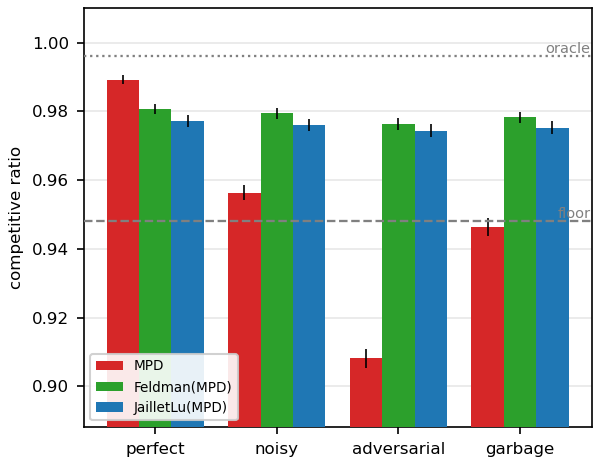
\includegraphics[width=\linewidth]{../../results/unified_benchmark_panelA.png}
\end{minipage}

\medskip
\noindent
\begin{minipage}[c]{0.60\linewidth}
\begin{tabular}{@{}lrrrr@{}}
\toprule
\emph{Panel B --- left-regular $d{=}5$} & perfect & noisy & advers. & garbage \\
\midrule
Greedy $=$ Ranking (floor) & 0.890 & --- & --- & --- \\
MinDegree (oracle) & 0.966 & --- & --- & --- \\
MPD & 0.932 & 0.906 & \textbf{0.854} & 0.888 \\
Feldman(MPD) & 0.906 & 0.903 & 0.896 & 0.900 \\
JailletLu(MPD) & 0.903 & 0.902 & 0.898 & 0.901 \\
Feldman (base) & 0.758 & --- & --- & --- \\
JailletLu (base) & 0.789 & --- & --- & --- \\
\bottomrule
\end{tabular}
\end{minipage}\hfill
\begin{minipage}[c]{0.38\linewidth}
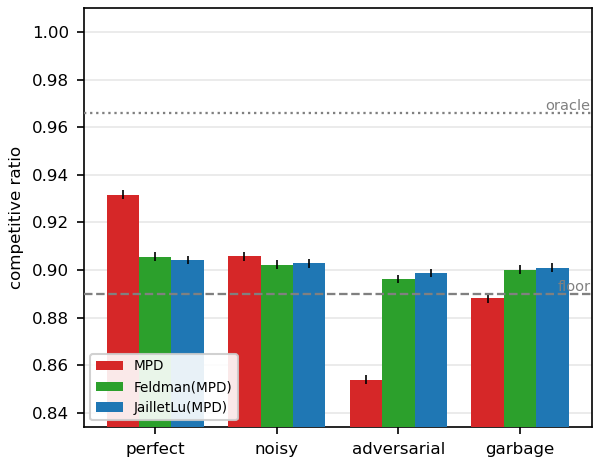
\includegraphics[width=\linewidth]{../../results/unified_benchmark_panelB.png}
\end{minipage}

\medskip
\noindent
\begin{minipage}[c]{0.60\linewidth}
\begin{tabular}{@{}lrrrr@{}}
\toprule
\emph{Panel C --- few-types $r{=}8$} & perfect & mild & bad & garbage \\
\midrule
Ranking (floor) & 0.990 & --- & --- & --- \\
MinDegree (oracle) & 0.999 & --- & --- & --- \\
FollowPrediction & 1.000 & 0.832 & 0.679 & \textbf{0.472} \\
TestAndMatch (Choo) & 1.000 & 0.984 & 0.989 & 0.990 \\
TestAndMatch (BEM) & 0.998 & 0.988 & 0.988 & 0.968 \\
Combiner \emph{(benchmark)} & 0.990 & 0.990 & 0.990 & 0.990 \\
\bottomrule
\end{tabular}
\end{minipage}\hfill
\begin{minipage}[c]{0.38\linewidth}
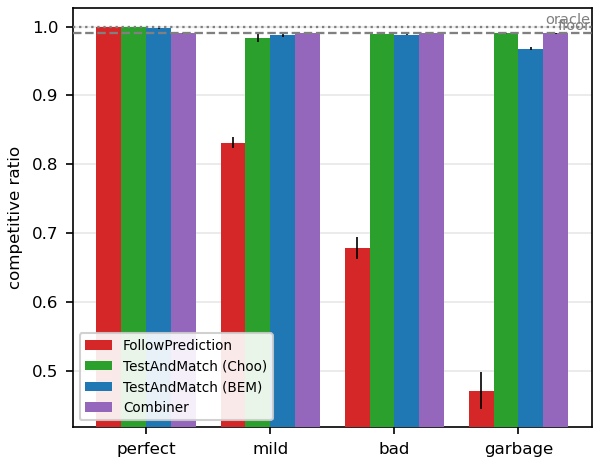
\includegraphics[width=\linewidth]{../../results/unified_benchmark_panelC.png}
\end{minipage}
\caption{The unified benchmark. Each panel's competitive ratios (means over paired
trials; every 95\% CI $\le 0.003$) sit beside their bar chart (error bars: 95\% CIs;
dashed line: advice-free floor; dotted: oracle ceiling). Bold marks dips below the
floor.}
\end{table}

\revpair{}{\revcard{revMust}{4-05 · R4 体例校对 · 必改 · 加粗规则与表注不符}{%
\textbf{原文}\hspace{0.4em}\textquotedblleft Bold marks dips below the floor\textquotedblright\par
\textbf{问题}\hspace{0.4em}表注说加粗表示跌破 floor，但 Panel C 的 floor 是 0.990，而 FollowPrediction 的 mild=0.832 和 bad=0.679 同样低于 floor，却只有 garbage=0.472 被加粗。规则和标记不一致，是考官翻表时最容易一眼看到的问题。\par
\textbf{建议}\hspace{0.4em}两个选择：把 Panel C 该加粗的三个数都加粗，或者把表注改成 bold marks each algorithm's worst column。无论选哪个，三个面板要用同一条规则。}
\revcard{revMust}{4-06 · R1 二审考官 · 必改 · 三个 floor 数值差异}{%
\textbf{原文}\hspace{0.4em}\textquotedblleft Ranking (floor) 0.948 / Greedy = Ranking (floor) 0.890 / Ranking (floor) 0.990\textquotedblright\par
\textbf{问题}\hspace{0.4em}同一张表里 floor 有三个值（0.948、0.890、0.990），第 6 章又出现 0.99 和 0.958。它们来自不同的图族，但表里没有任何提示，读者只会觉得数字对不上。这是全文一致性风险最高的一处（见 CROSS\_CHAPTER X-2）。\par
\textbf{建议}\hspace{0.4em}在表注加一句：the floor is instance-dependent; it is Ranking's ratio on that panel's own graph family。并回头统一第 6 章各处 floor 的写法与出处。}}

\section{4.2 Four findings}\label{four-findings}

\revpair{\textbf{(F1) Robustness is engineered, not free: naive followers crash
below the floor.} Both unguarded prediction-followers dive under the
advice-free Ranking floor once the prediction is adversarial or garbage:
MPD falls to \(0.908<0.948\) (Panel A) and \(0.854<0.890\) (Panel B),
and FollowPrediction collapses to \(0.472\ll0.990\) (Panel C). Using
either \emph{unguarded}\revhl{revMust}{is strictly worse than using no prediction at
all.}\revhlid{revMust}{4-07} Every robust algorithm --- the augmentations, TestAndMatch, the
combiner --- avoids this by construction.}{}

\revpair{\textbf{(F2) Two distinct robustness mechanisms, with different shapes.}
\emph{Structural} robustness (Feldman(MPD), JailletLu(MPD)): the
worst-case-optimal base matching carries the load and the prediction
only breaks ties, so performance is nearly \emph{flat} --- Feldman(MPD)
moves only \(0.981\!\to\!0.976\) from perfect to adversarial (Panel A).
It cannot crash but caps the upside (never reaching the \(0.996\)
oracle). \emph{Adaptive} robustness (TestAndMatch): test a sublinear
prefix, then commit --- capturing the upside when advice is good (Choo
\(1.000\)) and holding the floor when it is bad (\(0.990\)). On Panel C
it is the only algorithm on the upper envelope at both ends. The two
mechanisms trade consistency for robustness in opposite ways;
\textbf{Figure 4.1} plots every algorithm on the consistency--robustness
plane, where the opposite trades --- and the empty region beyond
TestAndMatch toward the ideal top-right corner --- are visible at a
glance.}{}

\revpair{\revfigure{../../results/consistency_robustness.png}{\revhl{revShould}{The consistency--robustness plane (the data of Table 4.1)}\revhlid{revShould}{4-08};
dashed lines mark the advice-free floor, dotted the oracle ceiling.
TestAndMatch sits nearest the ideal top-right corner.}}{\revcard{revMust}{4-07 · R2 领域审稿人 · 必改 · 断言范围}{%
\textbf{问题}\hspace{0.4em}strictly worse 是无条件断言，但同一张表里 MPD 在 perfect 和 noisy 两列都高于 floor（0.989 和 0.956 对 0.948）。这句话只在坏建议下成立。\par
\textbf{建议}\hspace{0.4em}补上条件：under adversarial or garbage advice, using either unguarded is worse than using no prediction at all。一个从句就把一句可被表格直接反驳的话救回来。}
\revcard{revShould}{4-08 · R1 二审考官 · 建议 · 图注不自足}{%
\textbf{问题}\hspace{0.4em}这是本章的总结图，图注却没说两个坐标轴各自怎么定义（consistency 用哪一列、robustness 用哪一列）。而这两个量的操作化定义正是 3.4 留下的问题。\par
\textbf{建议}\hspace{0.4em}图注写明：horizontal axis = ratio under perfect advice; vertical axis = ratio under the worst corruption level。读者才能自己核对点位。}}

\revpair{\textbf{(F3) The consistency upside is small on average-case inputs; the
spread lives on the bad-advice side.} On few-types \revhl{revShould}{the advice-free
Ranking is already}\revhlid{revShould}{4-10} \(0.990\) and MPD-with-true-degrees is \(0.999\) ---
under \(0.01\) for any advice to add on the good side. Every wide gap in
Panel C is a \emph{downside} gap. \revhl{revNice}{This is the thesis in one panel}\revhlid{revNice}{4-09};
Chapter 6 shows why no affordable test escapes it, and the concluding
outlook (§10.2) why it is forced.}{\revcard{revNice}{4-09 · R6 初次读者 · 可选 · 保持}{%
\textbf{问题}\hspace{0.4em}这句话是全章最好的一处指路，读者读到这里会立刻明白 Panel C 的地位。\par
\textbf{建议}\hspace{0.4em}保持。同类做法可以复制到第 6 章（哪一张图是那一章的题眼）和第 7 章。}
\revcard{revShould}{4-10 · R2 领域审稿人 · 建议 · 数值呈现}{%
\textbf{问题}\hspace{0.4em}0.01 这个上升空间是全文的核心量（10.2 的 stakes 就是它），但这里只作为一句顺带的减法出现，也没有给不确定度。既然每个数都有 CI，这个差值也应该有。\par
\textbf{建议}\hspace{0.4em}把它写成一个带不确定度的量：the entire consistency headroom is 0.009 +/- 0.00x - smaller than most of the effects we will measure。这一句会成为第 6 章和 10.2 反复引用的锚点。}}

\revpair{\textbf{(F4) The augmentation rescues structurally weak base
algorithms.} Feldman and Jaillet--Lu are tuned for the worst-case ratio
and are the \emph{weakest} advice-free entries on these average-case
inputs (Panel B: \(0.758\) / \(0.789\), below Greedy's \(0.890\)); the
MPD augmentation lifts them to \(\approx0.90\). The prediction does
\emph{more}\revhl{revShould}{for the worst-case-designed algorithms than for greedy --- a
pairing visible only under a unified table.}\revhlid{revShould}{4-11}}{\revcard{revShould}{4-11 · R5 答辩提问者 · 建议 · 自我表扬式断言}{%
\textbf{问题}\hspace{0.4em}visible only under a unified table 是对自己方法论的表扬，而且容易被反驳（分别做两组实验也能看到）。答辩现场这类句子是免费的靶子。\par
\textbf{建议}\hspace{0.4em}去掉 only：a pairing that a unified table makes immediate。观察本身很好，不需要这半句加分。}}

\section{4.3 Chapter summary}\label{chapter-summary}

\revpair{\revhl{revShould}{On average-case matching the advice-free baseline is already
near-optimal, unguarded prediction-following is unsafe, and the value of
the sophisticated algorithms is downside protection}\revhlid{revShould}{4-12} delivered by one of
two mechanisms. Chapters 5--7 sharpen each part --- what governs the
(small) loss, what the adaptive test costs, and whether the picture
survives on real data --- and the concluding outlook (§10.2) explains
why the wall is forced, not accidental.}{\revcard{revShould}{4-12 · R3 英语文字编辑 · 建议 · 小结与要点重复}{%
\textbf{问题}\hspace{0.4em}章末小结把 F1、F2、F3 又复述了一遍，而它们刚在两页前以加粗标题出现过。\par
\textbf{建议}\hspace{0.4em}小结只留一句本章结论加一句下章出口（第 5 章要问的是：这个小小的损失由什么决定）。}}

\chapter{\revhl{revShould}{Chapter 5. What Governs the Loss: Order Error and ACI's
Bound}\revhlid{revShould}{5-01}}\label{chapter-5.-what-governs-the-loss-order-error-and-acis-bound}

\revpair{Chapter 4 showed that on average-case inputs the loss of a
degree-prediction algorithm is small. This chapter asks what
\emph{governs} that loss. MinPredictedDegree matches by ascending
predicted degree, so it depends on the predictor \(\mu\) \emph{only
through the order it induces} on the resources: two predictors inducing
the same order produce identical matchings, and a monotone rescaling of
\(\mu\) changes nothing. The right question is therefore not ``how large
is the error'' but ``which \emph{order} error governs the loss, and how
tightly.'' Answering it requires care, because the qualitative fact that
order --- not magnitude --- matters is already a theorem, and we are
explicit about what is prior and what is ours.}{\revcard{revShould}{5-01 · R5 答辩提问者 · 建议 · 章标题}{%
\textbf{问题}\hspace{0.4em}这是全文唯一在章标题里放他人姓名缩写的章。ACI 对领域外读者是无意义的三个字母，而目录是考官最先看到的东西。\par
\textbf{建议}\hspace{0.4em}改成 Order Error and the Known Bound，或 Order Error: What the Known Bound Does and Does Not Say。归属留在正文（5.1 已经写得很好）。}}

\section{5.1 What is already known
(ACI)}\label{what-is-already-known-aci}

\revpair{Aamand, Chen and Indyk {[}@aci2022mpd, Appendix D{]} prove that on the
CLV-B model, MinPredictedDegree's matching loss relative to the true
expected degrees is at most \(n-\mathrm{LIS}(p[\mu])\), where \(p[\mu]\)
\revhl{revMust}{is the true weights ordered by}\revhlid{revMust}{5-02} \(\mu\) and \(\mathrm{LIS}\) is the
longest non-decreasing subsequence --- a pure \emph{order} quantity. In
particular a monotone (order-preserving) predictor has \(p[\mu]\)
already sorted, so \(n-\mathrm{LIS}=0\) and the loss is zero. Thus
\emph{order-dependence} and \emph{\revhl{revShould}{the zero-effect of a monotone bias}\revhlid{revShould}{5-03}}
are ACI's results, not ours; our \texttt{systematic\_bias} error model
(a monotone rescale) has Kendall-\(\tau\equiv0\) by construction and,
consistently, leaves MPD's ratio exactly unchanged across the benchmark
(Chapter 4) --- an empirical confirmation of ACI's statement, not a new
finding.}{\revcard{revMust}{5-02 · R4 体例校对 · 必改 · 符号冲突}{%
\textbf{问题}\hspace{0.4em}这里的 p 是真实权重向量，而 2.2、3.1 里的 p 是类型分布。同一篇论文用同一个字母指两个不同对象，并且都出现在讨论预测误差的语境中，第 5 章的核心公式因此可能被读错。\par
\textbf{建议}\hspace{0.4em}换字母：把真实权重写成 w，公式变成 n - LIS(w[mu])。改动很小，消除的是一个真实的误读风险。}
\revcard{revShould}{5-03 · R3 英语文字编辑 · 建议 · 免责声明重复}{%
\textbf{问题}\hspace{0.4em}本章在 5.1 末、5.2 开头、5.3 开头三次声明这不是我们的发现。诚实是对的，但三次会变成过度自我设限，读者反而记不住本章真正的贡献。\par
\textbf{建议}\hspace{0.4em}保留 5.1 末的这一处（它在证据旁边，最有说服力），5.3 改成正面陈述本章加了什么，把 not ours 压缩成半句。}}

\section{5.2 Our characterization}\label{our-characterization}

\revpair{We sweep the four structured error models across strength and record,
per model and level on the same instances, three quantities: the actual
MPD matching loss, ACI's \(n-\mathrm{LIS}\), \revhl{revShould}{and the normalized
Kendall}\revhlid{revShould}{5-04}-\(\tau\) order error (\textbf{Figure 5.1}; \(n=1000\), Zipf
exponent \(1.0\), 40 trials).}{\revcard{revShould}{5-04 · R1 二审考官 · 建议 · 度量未定义}{%
\textbf{问题}\hspace{0.4em}normalized 的归一化方式没说：0 表示完全一致、1 表示完全反序吗；还是 1 减去相关系数。全章的结论都挂在这个量上，第 7 章还要拿它跨数据集比较。\par
\textbf{建议}\hspace{0.4em}给出定义式或一句话：we report tau normalized to [0,1], where 0 means the predicted order is exactly right and 1 means it is exactly reversed。}}

\revpair{\revfigure{../../results/order_vs_theory.png}{Order error governs the loss: the realized loss lies far below
ACI's \(n-\mathrm{LIS}\) bound (a) and collapses onto Kendall-\(\tau\)
across all four error models (b).}}{}

\revpair{\textbf{(i) ACI's \(n-\mathrm{LIS}\) bound is correct but very loose.}
\revhl{revShould}{The realized loss lies far below the bound at every point --- by roughly}\revhlid{revShould}{5-05}
\(16\times\) (adversarial) to \(75\times\) (distribution-drift); all
points hug the axis in Figure 5.1(a).}{\revcard{revShould}{5-05 · R2 领域审稿人 · 建议 · 倍数的算法}{%
\textbf{问题}\hspace{0.4em}16 倍和 75 倍是怎么算的没有说明：是 bound 除以 loss 的均值，还是在某个特定误差强度上取的比。松紧程度是本章贡献之一，读者需要能复核。\par
\textbf{建议}\hspace{0.4em}写明口径：ratio of the bound to the realized loss, at the strongest corruption level of each model（或你实际用的口径）。}}

\revpair{\textbf{(ii) \(n-\mathrm{LIS}\) saturates and cannot distinguish error
structures.} \revhl{revShould}{For every non-trivial error it is pinned near its maximum}\revhlid{revShould}{5-06}
(\(\approx610\)--\(673\) for \(n=1000\)), even though the true losses
differ by a factor of five across models (\(8.1\) drift, \(21.6\)
random-flip, \(41.7\) adversarial). As a bound that is almost always
\(\approx n\), it carries little information about which prediction is
more harmful.}{\revcard{revShould}{5-06 · R2 领域审稿人 · 建议 · 饱和的证据}{%
\textbf{问题}\hspace{0.4em}饱和这个结论用了一个区间（610 到 673），但没给最大可能值。读者要自己推断 n - LIS 的上界是不是 n = 1000，从而判断 610 到 673 算不算贴顶。\par
\textbf{建议}\hspace{0.4em}补一句参照：out of a maximum of n = 1000, and against realized losses of 8 to 42。三个量放在一起，饱和这个结论才立得住。}}

\revpair{\textbf{(iii) Kendall-\(\tau\) is the governing order measure, and the
models collapse onto it.} Plotted against Kendall-\(\tau\) (Figure
5.1(b)), \revhl{revMust}{the four models fall on one increasing curve}\revhlid{revMust}{5-07} --- loss rises
with \(\tau\) (\(0.29\to0.50\to1.0\) for drift, random-flip,
adversarial, tracking \(8.1\to21.6\to41.7\)), with
\texttt{systematic\_bias} pinned at \(\tau=0\), zero loss. The quantity
that \emph{predicts} the loss and unifies the error structures is the
Kendall-\(\tau\) order distance, which the saturated \(n-\mathrm{LIS}\)
cannot resolve.}{\revcard{revMust}{5-07 · R2 领域审稿人 · 必改 · 视觉断言缺量化}{%
\textbf{问题}\hspace{0.4em}这是本章最重要的正面结论（Kendall-tau 是统一四个误差结构的量），但支撑它的只有一句对图的目视描述。审稿人会立刻要一个数：单调性有多强、四个模型的点重合到什么程度。\par
\textbf{建议}\hspace{0.4em}给一个统计量：例如四个模型合并后的 Spearman 相关系数，或以 tau 为唯一自变量拟合后的 R\textasciicircum{}2 与各模型残差。一个数就能把目视断言变成可核查的结果。}}

\section{\revhl{revShould}{5.3 Chapter summary}\revhlid{revShould}{5-08}}\label{chapter-summary}

\revpair{We do not claim that order rather than magnitude governs MPD --- ACI's
Appendix D establishes that, along with the zero-effect of a monotone
bias. What we add is a precise empirical characterization: ACI's
\(n-\mathrm{LIS}\) bound is loose by one to nearly two orders of
magnitude and saturates, whereas Kendall-\(\tau\) predicts the realized
loss and unifies the four error structures. This both sharpens the
theory's practical content and justifies the single order-error axis
used when the predictor is stressed on real data (Chapter 7).}{\revcard{revShould}{5-08 · R6 初次读者 · 建议 · 章太短且无出口}{%
\textbf{问题}\hspace{0.4em}全章只有三页，且小结没有说明第 5 章的结论会在哪里被用到（第 7 章用它解释为什么廉价预测器有效、第 8 章用它推出排序学习的想法）。这个因果链是全文最漂亮的一条，值得点破。\par
\textbf{建议}\hspace{0.4em}小结加一句出口：this is why Chapter 7 can explain a cheap predictor's success by its order fidelity, and why Chapter 8 tried to train for order directly。}}

\chapter{Chapter 6. Test-and-Fallback in
Depth}\label{chapter-6.-test-and-fallback-in-depth}

\revpair{The test-and-fallback algorithms are the adaptive robustness mechanism
of Chapter 4. \revhl{revShould}{This chapter gives their first empirical study: the
robustness envelope they achieve}\revhlid{revShould}{6-02} (§6.1), a counter-intuitive failure of
the acceptance threshold (§6.2), its recalibration and the resolution
limit that recalibration exposes (§6.3) --- a limit that persists across
the whole difficulty range and anchors the theoretical outlook of §10.2
--- and a benchmark of the dynamic combiner that explains the
\emph{commit-once} structure (§6.4). Throughout, the \(\ell_1\) test is
the empirical surrogate the original authors also fall back to (Chapter
3).}{\revcard{revMust}{6-01 · R1 二审考官 · 必改 · 名称未消歧}{%
\textbf{问题}\hspace{0.4em}本章有四个名字在流通：FollowPrediction、TestAndMatch、Choo、BEM。前两个是策略名，后两个是作者缩写，但正文从未说明 Choo 和 BEM 是同一个 TestAndMatch 的两种变体、还是两个不同算法。6.1 直接写 BEM 0.998 到 0.969；Choo 1.000 到 0.991，读者到这里必须自己反推。\par
\textbf{建议}\hspace{0.4em}在本章导语加一句名称表：we write TestAndMatch for the test-and-fallback scheme in general, and Choo and BEM for its two published instantiations, which differ only in the acceptance threshold。四个名字一次说清，全章受益。}
\revcard{revShould}{6-02 · R3 英语文字编辑 · 建议 · 导语长句}{%
\textbf{问题}\hspace{0.4em}一句 70 词，四项并列，中间还插了一个破折号从句。章导语是读者决定怎么读这一章的地方，恰恰最不该长。\par
\textbf{建议}\hspace{0.4em}拆成两句：一句列四项（各一个短语），一句单独说 6.3 的分辨率极限是本章通往 10.2 的接口。}}

\section{6.1 The robustness envelope}\label{the-robustness-envelope}

\revpair{\revhl{revShould}{Sweeping advice error}\revhlid{revShould}{6-03} \(\ell_1(p,q)\) on few-types instances
(\(n=2000\), \(r=8\), prefix \(k=200\), 40 trials; \textbf{Figure 6.1}),
FollowPrediction degrades \emph{linearly} from \(1.000\) at perfect
advice to \(0.453\) at \(\ell_1\!\approx\!1.1\) --- well \emph{below}
the advice-free floor (\(\approx0.99\)). \revhl{revMust}{TestAndMatch instead stays on
the}\revhlid{revMust}{6-01} \textbf{upper envelope}: it captures the benefit when advice is good
and, when advice is bad, \revhl{revShould}{its prefix test rejects it and it falls back to
Ranking, never crashing}\revhlid{revShould}{6-04} (BEM \(0.998\to0.969\); Choo \(1.000\to0.991\)).
This is the adaptive counterpart of the structural robustness of Chapter
4.}{\revcard{revShould}{6-03 · R1 二审考官 · 建议 · 符号未复述}{%
\textbf{问题}\hspace{0.4em}四个符号在第 3 章定义，但读者到这里已经隔了十五页，尤其 r 和 k 很容易记混（r 是类型数还是资源数？k 是前缀长度还是折数？）。\par
\textbf{建议}\hspace{0.4em}括号里就地补词：(n=2000 arrivals, r=8 request types, a prefix of k=200 arrivals, 40 trials)。多几个词，读者不用回翻。}
\revcard{revShould}{6-04 · R2 领域审稿人 · 建议 · 全称断言}{%
\textbf{问题}\hspace{0.4em}never 是全称量词，而证据是一条误差 sweep、一个图族、40 次重复。审稿人会盯这类词。\par
\textbf{建议}\hspace{0.4em}限定到证据范围：it does not fall below the advice free floor at any point of this sweep。真正的全称结论留给 6.3 的机制解释去承担。}}

\revpair{\revfigure{../../results/choo_bem_envelope.png}{The robustness envelope: blind FollowPrediction crashes below
the advice-free floor as advice error grows; TestAndMatch stays on the
upper envelope.}}{}

\section{6.2 A threshold that is too lenient on average-case
inputs}\label{a-threshold-that-is-too-lenient-on-average-case-inputs}

\revpair{Sweeping the prefix (testing) size \(k\) at \emph{borderline} advice
(\(\eta=0.15\), true \(\ell_1\!\approx\!0.16\)) --- where the test works
hardest (\textbf{Figure 6.2}) --- a larger, more accurate test makes the
\emph{worse} decision: as \(k\) grows \(25\to800\), the ratio
\emph{falls} \(0.992\to0.956\) and the misjudgement rate \emph{rises}
\(0.00\to0.60\). The mechanism: the Choo/BEM threshold \(\tau\) \revhl{revMust}{is
calibrated to the worst-case baseline}\revhlid{revMust}{6-05} \(\beta\approx0.696\), but on
these instances the baseline is \(\approx0.99\) (F3), so the empirical
break-even sits at \(\ell_1\approx0\), far below \(\tau\). A small noisy
prefix over-estimates \(\ell_1\) and \emph{accidentally rejects} the
borderline advice \revhl{revShould}{(landing safely on the floor)}\revhlid{revShould}{6-08}; a large accurate prefix
correctly measures \(\ell_1\approx0.16<\tau\) and \emph{accepts}\revhl{revMust}{the
mildly-bad advice}\revhlid{revMust}{6-06}the worst-case threshold deems acceptable ---
underperforming the baseline. On strong-baseline inputs the worst-case
threshold is too lenient, and a more accurate test only follows it more
faithfully.}{\revcard{revMust}{6-05 · R1 二审考官 · 必改 · 数字来源缺失}{%
\textbf{问题}\hspace{0.4em}0.696 凭空出现。读者（尤其二审）会立刻想：这个数是哪来的、为什么不是 1-1/e。这是本节机制解释的支点，支点没有来源，整个 pathology 的论证就悬空了。\par
\textbf{建议}\hspace{0.4em}补半句出处：beta is the worst case competitive ratio the advice free baseline is proved to achieve in this model (see 2.x / the original paper)。若是你自己算的，写明算法与实例族。}
\revcard{revMust}{6-06 · R3 英语文字编辑 · 必改 · 信息密度}{%
\textbf{问题}\hspace{0.4em}一段里有六组数字加一条两步机制解释，其中一句 45 词。这是全章最反直觉的发现，却是最难读的一段，第一次读需要读三遍。\par
\textbf{建议}\hspace{0.4em}改成三段式：第一句只讲现象（更大的测试反而做出更差的决定，给两个数）。第二句讲原因的一半（阈值是按最坏情况基线校准的，而这些实例的基线是 0.99）。第三句讲另一半（小前缀因为噪声误拒而侥幸安全，大前缀准确测量后照章接受了坏建议）。数字各归各句。}}

\revpair{\mbox{}}{\revcard{revShould}{6-07 · R3 英语文字编辑 · 建议 · 强调过密}{%
\textbf{原文}\hspace{0.4em}\textquotedblleft worse / falls / rises / accidentally rejects / accepts / below\textquotedblright\par
\textbf{问题}\hspace{0.4em}这一段有八处斜体强调。强调密度一高，强调就失效，读者反而抓不到哪个才是重点。\par
\textbf{建议}\hspace{0.4em}每段最多留一到两处。本段真正需要强调的只有一个词组：more accurate 却 worse decision。}
\revcard{revShould}{6-08 · R6 初次读者 · 建议 · 题眼被藏起来}{%
\textbf{问题}\hspace{0.4em}错误的原因导致了正确的结果，这是本节最有意思、也最能体现你观察力的一点，现在被塞在括号里一带而过。\par
\textbf{建议}\hspace{0.4em}把它提成独立一句并点名：the small test is right for the wrong reason - it rejects because it is noisy, not because the advice is bad。这句话会成为读者记住这一节的抓手。}}

\revpair{\revfigure{../../results/choo_bem_prefix.png}{Testing cost at borderline advice: a larger, more accurate
prefix test makes the \emph{worse} decision under the
worst-case-calibrated threshold.}}{}

\section{\revhl{revMust}{6.3 Recalibration, and the resolution limit it
exposes}\revhlid{revMust}{6-09}}\label{recalibration-and-the-resolution-limit-it-exposes}

\revpair{Recalibrating \(\tau\) to the \emph{measured} baseline \(\hat\beta\)
eliminates the pathology (\textbf{Figure 6.3}): at borderline advice the
worst-case threshold's misjudgement climbs \(0.03\to1.00\) as the prefix
grows and its ratio drops to \(0.920\), while the recalibrated threshold
holds misjudgement \(0.00\) at every prefix and ratio \(\approx0.986\).
But recalibration exposes a deeper limit. At perfect advice the
worst-case threshold scores \(1.000\) while the recalibrated one scores
only \(0.987\): the recalibrated
\(\tau\approx2(1-\hat\beta)\approx0.028\) is \emph{smaller than the
empirical-\(\ell_1\) \revhl{revShould}{estimator's noise floor}\revhlid{revShould}{6-12}}
(\(\approx0.05\)--\(0.13\)), so it can never confidently \emph{accept}
--- it rejects everything, including perfect advice, and always plays
the baseline. In short:}{}

\revpair{\begin{quote}
\revhl{revShould}{On strong-baseline instances, no practical}\revhlid{revShould}{6-10} empirical-\(\ell_1\)
threshold can both capture the consistency upside and stay safe: the
upside is tiny and sits \emph{below the estimator's resolution}. The
worst-case threshold over-accepts; the recalibrated one over-rejects; \revhl{revShould}{a
better tester only follows whichever threshold more faithfully}\revhlid{revShould}{6-11}.
\end{quote}}{\revcard{revMust}{6-09 · R1 二审考官 · 必改 · 先用后释}{%
\textbf{问题}\hspace{0.4em}resolution limit 出现在节标题里，正文到第六行才隐含解释（阈值小于估计量噪声底）。读者带着一个没定义的词读了半页。\par
\textbf{建议}\hspace{0.4em}节的第一句就下定义：by resolution we mean the smallest difference in ell\_1 the empirical estimator can distinguish from noise at prefix length k。后面的论证才有依托。}
\revcard{revShould}{6-10 · R2 领域审稿人 · 建议 · 断言范围}{%
\textbf{问题}\hspace{0.4em}no ... can 是不可能性断言，而证据是两个具体阈值加一次噪声底估计。practical 和 empirical-ell\_1 这两个限定词已经做得很好，但审稿人仍会问：所有阈值都试过了吗。\par
\textbf{建议}\hspace{0.4em}把量词落到证据上：among thresholds of this form, and at the prefix lengths we can afford, none both captures ... 真正的任意规则版本是 10.2 的事，两处的强度要分开。}}

\revpair{\mbox{}}{\revcard{revShould}{6-11 · R3 英语文字编辑 · 建议 · 重复}{%
\textbf{问题}\hspace{0.4em}与 6.2 末句 a more accurate test only follows it more faithfully 几乎同形同义，隔了半页再说一遍，第二次读起来像作者忘了自己写过。\par
\textbf{建议}\hspace{0.4em}6.2 那句改成机制描述，把这句金句留给 6.3 的小结独享。}
\revcard{revShould}{6-12 · R2 领域审稿人 · 建议 · 估计量缺说明}{%
\textbf{问题}\hspace{0.4em}噪声底给了区间但没说这个区间是怎么来的、随什么变化（k？r？重复次数？）。这是本节论证的关键量，也是整篇论文通往 10.2 的桥。\par
\textbf{建议}\hspace{0.4em}补一句：the range spans k from 25 to 800 (noise falls as k grows); it is the standard deviation of the plug in estimate across trials at zero true error。一句话就把这个数从断言变成可复核的量。}}

\revpair{\revfigure{../../results/recalibration_prefix.png}{Recalibration removes the threshold pathology: misjudgement
holds at zero at every prefix size, versus climbing toward \(1.0\) under
the worst-case threshold.}}{}

\revpair{\textbf{Figure 6.4} widens this finding from one threshold to the whole
difficulty range. Sweeping the number of types --- the knob that sets
the baseline strength --- the \emph{potential} upside of perfect advice
grows as the baseline weakens, but the upside a sublinear-prefix test
can \emph{safely capture} stays pinned near zero: the empirical test's
resolution (its noise floor) sits far above the break-even margin
wherever an upside exists. The wall of this chapter is therefore not one
badly calibrated threshold. The upside and the testing resolution move
together --- and the concluding outlook (§10.2) gives this coupling a
quantitative form: the prefix needed to decide scales as the inverse
square of the stakes.}{}

\revpair{\revfigure{../../results/impossibility_frontier.png}{The testing-wall frontier: \revhl{revShould}{as the baseline weakens (left)}\revhlid{revShould}{6-13}, the
\emph{potential} upside of perfect advice grows, but the upside a
sublinear test can \emph{safely capture} stays near zero --- the
empirical test's resolution sits far above the break-even margin
wherever the upside exists.}}{\revcard{revShould}{6-13 · R1 二审考官 · 建议 · 图注不自足}{%
\textbf{问题}\hspace{0.4em}这是全章最重要的一张图，图注却没说横轴是什么。as the baseline weakens (left) 只是暗示了方向，读者要回正文才知道扫的是类型数 r。图应当能脱离正文被看懂。\par
\textbf{建议}\hspace{0.4em}图注首句直接交代坐标：horizontal axis: number of request types r (fewer types = weaker advice free baseline, shown left); vertical axis: ratio gain over the baseline。然后再讲结论。}}

\section{6.4 The dynamic combiner is dominated, and shows why matching
needs
test-then-commit}\label{the-dynamic-combiner-is-dominated-and-shows-why-matching-needs-test-then-commit}

\revpair{We benchmark the Chłędowski-style dynamic combiner to contextualize the
commit-once structure of test-and-fallback. \revhl{revMust}{In its robust tuning the
combiner sits exactly on the floor}\revhlid{revMust}{6-15} (\(0.990\) across all advice
quality): it never crashes but captures none of the consistency upside,
strictly dominated by TestAndMatch. More instructively, an \emph{eager}
combiner that switches mid-stream reveals a penalty specific to
irrevocable problems: with perfect advice, \revhl{revMust}{eager switching scores}\revhlid{revMust}{6-14}
\(0.927\) --- \emph{below both} the pure follower (\(1.000\)) and the
pure baseline (\(0.958\); \texttt{tests/test\_combiner\_small.py}) ---
because \revhl{revShould}{switching from Ranking to advice-following (}\revhlid{revShould}{6-16}\emph{mimic})
mid-run lands the committed matching in an \emph{incompatible hybrid}.
In an irrevocable problem the follow/fallback decision must be made
\emph{before} the bulk of the commitments, which is why Choo/BEM test a
prefix and then \emph{commit} rather than switching dynamically. The
dynamic combiner that is cheap insurance for caching does not port
cleanly to matching.}{\revcard{revMust}{6-14 · R5 答辩提问者 · 必改 · 数据来源可疑}{%
\textbf{问题}\hspace{0.4em}论文正文的数字引用了一个单元测试文件。答辩时这一定会被问：这是正式实验还是小规模自测、n 多大、重复多少次、有没有置信区间。全章其他数字都有实验设置，只有这一处没有。\par
\textbf{建议}\hspace{0.4em}要么把它升级为一次正式实验并给出与 6.1 同格式的设置与置信区间，要么在正文明说它的地位：a small scale sanity experiment (n=..., ... trials), reported to illustrate the mechanism rather than to measure it。脚本路径移到附录 A 的映射表里。}
\revcard{revMust}{6-15 · R4 体例校对 · 必改 · 同名不同值}{%
\textbf{问题}\hspace{0.4em}本章出现了三个都叫基线或 floor 的数：0.99、0.990、0.958。它们大概来自不同实例族与不同规模，但正文没有区分，读者只会认为哪里算错了。这是最容易被考官当场指出的不一致。\par
\textbf{建议}\hspace{0.4em}两条都做：给每个数标注它所在的实例设置（一个括号即可），并在本章第一次出现时统一命名（advice free floor 只指 6.1 那个族的数）。若三者本可统一，那就统一。}}

\revpair{\mbox{}}{\revcard{revShould}{6-16 · R4 体例校对 · 建议 · 代码名进正文}{%
\textbf{问题}\hspace{0.4em}mimic 是代码里的策略名，在正文这是它第一次也是唯一一次出现，读者不知道它和 advice following 是不是两回事。\par
\textbf{建议}\hspace{0.4em}删掉 mimic，或写成 (called mimic in the implementation)。正文只用一个名字。}}

\section{6.5 Chapter summary}\label{chapter-summary}

\revpair{Test-and-fallback delivers the adaptive robustness envelope of §6.1, but
its accept/reject decision is fundamentally limited on strong-baseline
inputs: no empirical-\(\ell_1\) threshold both captures the upside and
stays safe (§6.3), and dynamic switching is dominated by
test-then-commit (§6.4). \revhl{revNice}{The resolution limit of}\revhlid{revNice}{6-17} §6.3 --- and its
persistence across the whole difficulty range (Figure 6.4) --- is the
empirical anchor of the theoretical outlook in §10.2.}{\revcard{revNice}{6-17 · R6 初次读者 · 可选 · 小结无出口}{%
\textbf{问题}\hspace{0.4em}本章小结只回顾结论，没有告诉读者接下来该带着什么问题读第 7 章。全书各章小结的结构如果一致（回顾 + 出口），阅读节奏会好很多。\par
\textbf{建议}\hspace{0.4em}末尾补一句出口：the next chapter asks whether this picture survives outside synthetic instances。并检查其他各章小结是否都有这样一句。}}

\chapter{Chapter 7. External
Validity}\label{chapter-7.-external-validity}

\revpair{\revhl{revShould}{Chapters 4--6 use synthetic graphs and a synthetic error knob. Is the
picture real? We stress it three ways}\revhlid{revShould}{7-01}: a genuine, cheap predictor on a
real request trace (§7.1); the six real-world graphs (§7.2); and whether
\emph{learning} the predictor changes anything (§7.3).}{\revcard{revShould}{7-01 · R1 二审考官 · 建议 · 外部效度的口径}{%
\textbf{问题}\hspace{0.4em}本章开门见山很好，但没说清楚三种压力测试各自替换掉了哪一个合成成分（预测误差来源、图、预测器的训练方式）。读者读完三节后才拼得出来。\par
\textbf{建议}\hspace{0.4em}在这句后加一句对照：7.1 replaces the synthetic error with real drift, 7.2 replaces the synthetic graphs with real ones, 7.3 replaces the hand-made predictor with a learned one。一句话给出本章的骨架。}}

\section{7.1 A real, cheap predictor}\label{a-real-cheap-predictor}

\revpair{We replace the synthetic knob with the cheapest realistic predictor:
last-window historical statistics. Real Wikipedia daily pageviews give a
live day (the truth) and earlier days (a 1-, 7-, or 30-day-stale
forecast), so the error is genuine temporal drift; \revhl{revShould}{we map the trace onto
a fixed serving topology and consume the forecast through the degree
route}\revhlid{revShould}{7-05} (MPD) (\textbf{Figure 7.1}). \revhl{revMust}{Three facts emerge}\revhlid{revMust}{7-02}. First,
\textbf{\revhl{revShould}{the cost premise does not bite}\revhlid{revShould}{7-04}}: the predictor is a linear-time
count (\(0.108\) ms --- about \(2\%\) of computing \(\mathrm{OPT}\)
once), not an ML inference. Second, \textbf{the benefit is real,
partial, and never harmful}: \revhl{revMust}{a stale forecast captures}\revhlid{revMust}{7-03}
\(27\%\)--\(68\%\) of the oracle gap (falling with staleness) and always
stays above the baseline (\(0.938\)--\(0.957\) vs \(0.923\)--\(0.925\),
even at 30 days). Third, and why: \textbf{topology aggregation makes the
cheap predictor order-faithful} --- the induced degree predictor's order
error is only Kendall-\(\tau\approx0.19\)--\(0.32\), roughly \emph{half}
the raw histogram's (\(0.38\)--\(0.49\)) --- and since MPD depends only
on order (Chapter 5), the aggregated route survives real drift.
Consuming the \emph{same} forecast through the raw histogram is
catastrophic: blind FollowPrediction collapses to \(0.68\to0.36\), far
below the \(\approx0.92\) baseline --- exactly what the robust
algorithms of Chapters 4 and 6 are for.}{\revcard{revMust}{7-02 · R3 英语文字编辑 · 必改 · 单段承载过多}{%
\textbf{问题}\hspace{0.4em}7.1 是一段 15 行，装了三个发现、每个发现两到三个数字、一条机制解释和一个反例。这是全章最有说服力的一节，也是最难读的一节。\par
\textbf{建议}\hspace{0.4em}拆成三段（每个 fact 一段），机制解释单独一段。数字保留，但每段只留最能说明问题的那一个。}
\revcard{revMust}{7-03 · R1 二审考官 · 必改 · 指标未定义}{%
\textbf{问题}\hspace{0.4em}gap-capture 这个指标在这里第一次出现且没有定义（应是算法相对基线的提升除以 oracle 相对基线的提升）。它随后在 8.1 又用了一次，是本文用来讲小上升空间的主力指标。\par
\textbf{建议}\hspace{0.4em}就地给定义式：we report gap-capture, (ALG - baseline)/(oracle - baseline)。一行公式，全文两处受益。}}

\revpair{\mbox{}}{\revcard{revShould}{7-04 · R1 二审考官 · 建议 · 术语自造}{%
\textbf{问题}\hspace{0.4em}cost premise 是本文自造的说法，指的大概是带预测算法默认预测器很贵这个前提，但正文从未提出过这个前提。读者不知道在反驳谁。\par
\textbf{建议}\hspace{0.4em}先把前提写出来再打掉：the with-predictions literature usually assumes the predictor is an expensive model; here it is a linear-time count（并给出那 0.108 毫秒作为证据）。}
\revcard{revShould}{7-05 · R1 二审考官 · 建议 · 实验设置缺失}{%
\textbf{问题}\hspace{0.4em}这个映射是本节外部效度的关键一步（真实 trace 怎么变成二部图），却只有半句。读者无法判断结论有多少来自真实数据、多少来自映射方式的选择。\par
\textbf{建议}\hspace{0.4em}补两句说明映射规则，或指向附录 A.5；并说明映射方式的选择是否影响结论（是否试过别的映射）。}}

\revpair{\revfigure{../../results/real_predictor.png}{A real, cheap predictor (Wikipedia trace): the aggregated
degree route survives staleness (b) because aggregation halves the order
error (a); blind histogram-following decays.}}{}

\section{7.2 Six real-world graphs}\label{six-real-world-graphs}

\revpair{We re-run the degree-prediction roster of Chapter 4 on the six
Network-Repository graphs (two Facebook social, two C. elegans
biological, two economic input-output), across the same quality columns,
with 95\% CIs (\textbf{Figure 7.2}). The two load-bearing findings are
universal. \textbf{F1 holds on all six}: naive MPD fed an adversarial
predictor falls \revhl{revShould}{below the Ranking floor everywhere}\revhlid{revShould}{7-09} --- by \(0.07\)
(Caltech36) to \(0.11\) (CE-PG). \textbf{\revhl{revMust}{F3 is universal and confirms
its own logic}\revhlid{revMust}{7-06}}: the consistency upside is small everywhere (mean
\(+0.049\); range \(+0.022\)--\(+0.077\)) and smallest exactly where the
baseline is strongest --- the two dense economic graphs, with Ranking
already \(0.965\)/\(0.977\), give the tiniest upsides.}{\revcard{revMust}{7-06 · R2 领域审稿人 · 必改 · 断言过强}{%
\textbf{问题}\hspace{0.4em}universal 用在六个图的样本上过强，尤其本节紧接着就要说 F2 在其中两个图上只是部分成立。审稿人会抓这个词。\par
\textbf{建议}\hspace{0.4em}改成 holds on all six graphs we tested，并把机制解释（上升空间在基线最强处最小）留作真正的论点 - 那才是这一节的价值。}
\revcard{revShould}{7-07 · R2 领域审稿人 · 建议 · 判据不对称}{%
\textbf{问题}\hspace{0.4em}strictly 给了判据（spread 倍数），qualitatively 没有。两个词并列出现却只有一个可核查，读者会怀疑 qualitatively 是不是事后放宽的口径。\par
\textbf{建议}\hspace{0.4em}给出 qualitatively 的判据：例如 the augmentations' spread is smaller than naive MPD's on all six。两个判据都写死。}}

\revpair{The structural-robustness finding \textbf{\revhl{revShould}{F2 holds qualitatively on all
six}\revhlid{revShould}{7-07}} (the augmentations are always less sensitive to prediction quality
than naive MPD) and \emph{strictly} on the four social/bio graphs
(spread \(0.22\)--\(0.29\times\) MPD's); on the two dense economic
graphs the protection is only \emph{partial} --- the augmentation
cushions the adversarial drop (\(0.939\) vs naive MPD's \(0.893\)) but
cannot clear the unusually high \(0.965\) floor, dipping \(\approx0.03\)
below it. \revhl{revMust}{This econ boundary is instructive rather than a failure}\revhlid{revMust}{7-08}: those
graphs are so dense that matching is nearly trivial (Ranking
\(\approx0.97\), MinDegree \(=1.00\)), so there is neither upside to
capture (F3) nor much downside to protect. Finally, F4 is
\emph{dramatic}: the worst-case-designed Feldman/Jaillet--Lu are the
weakest advice-free entries on the econ graphs (\(0.73\)--\(0.77\)) and
the augmentation lifts them to \(0.99\) --- a \(+0.26\) rescue.}{\revcard{revMust}{7-08 · R5 答辩提问者 · 必改 · 自我辩护}{%
\textbf{问题}\hspace{0.4em}遇到不利结果时先给自己定性（不是失败），是审稿人和考官最敏感的写法之一，反而会让人多看两眼这个边界。后面的解释（图太密、匹配近乎平凡）本身是充分的。\par
\textbf{建议}\hspace{0.4em}删掉这句评价，直接给解释和它的含义：on these two graphs matching is nearly trivial, so there is neither upside to capture nor downside to protect - the mechanism, not an exception。让读者自己得出不是失败的结论。}
\revcard{revShould}{7-09 · R1 二审考官 · 建议 · 图注不自足}{%
\textbf{问题}\hspace{0.4em}图注用颜色指代算法（red / green / blue），但没有说明六个子图的排布和纵轴范围是否统一。六联图如果纵轴不同，跨图比较就是错的。\par
\textbf{建议}\hspace{0.4em}图注写明：one panel per graph, shared vertical axis (or: axes differ; see values in text)。这一句决定了读者能不能横向读这张图。}}

\revpair{\revfigure{../../results/realworld_robustness.png}{F1--F3 on six real graphs: naive MPD (red) dips below the
Ranking floor everywhere; the structural augmentations (green/blue) stay
flat.}}{}

\section{7.3 Does learning the predictor
help?}\label{does-learning-the-predictor-help}

\revpair{Because MPD consumes the predictor only through order (Chapter 5), one
might train it with a rank loss rather than regression. We tested this
and report an honest negative. With \emph{deliberately divergent}
\revhl{revMust}{synthetic features rank-training beats regression sharply}\revhlid{revMust}{7-10}
(\(0.989\approx\) oracle vs \(0.974\), with worse regression error but
better order); but the advantage is gated by feature divergence and by
graph difficulty (peaking at \(+1.3\%\)), and, decisively, on real
temporal features it \emph{disappears} --- rank- and regression-trained
predictors produce identical order (Kendall-\(\tau\) \(0.126\) vs
\(0.126\)) and identical ratio. The dissociation that powers order-aware
training is a property of engineered features, not realistic ones. (The
fuller account of this exploration is Chapter 8.) The lesson reinforces
the thesis: once a predictor is order-faithful --- which a cheap
historical count already is (§7.1) --- neither a better algorithm nor a
better-trained predictor buys much on average-case matching.}{\revcard{revMust}{7-10 · R4 体例校对 · 必改 · 跨章重复}{%
\textbf{问题}\hspace{0.4em}7.3 与 8.1 讲的是同一组实验、同一批数字（0.989 / 0.974 / 0.126），两处各写一遍。读者读到第 8 章会以为是新实验，核对后发现是同一个。\par
\textbf{建议}\hspace{0.4em}定正本：第 8 章是正本（那里有完整的 M0 到 M3 过程），7.3 压到三句并明确写 the full account is in 8.1。或者反过来，但不要两处都是完整版。}}

\section{7.4 Chapter summary}\label{chapter-summary}

\revpair{\revhl{revShould}{On real predictors, real graphs, and a learned predictor, the same wall
stands}\revhlid{revShould}{7-11}: the advice-free baseline is near-optimal, unguarded following is
unsafe, and predictions buy downside protection rather than performance.
Having established the wall empirically across every setting we could
reach, Chapter 8 reports the directions that tried to get past it, and
the concluding outlook (§10.2) explains why it is forced.}{\revcard{revShould}{7-11 · R6 初次读者 · 建议 · 章末口径}{%
\textbf{问题}\hspace{0.4em}小结把三节压成一句，很好；但 7.2 那两个 econ 图上 F2 只是部分成立的事实在小结里消失了。考官若先读小结再回看正文，会觉得小结报喜不报忧。\par
\textbf{建议}\hspace{0.4em}小结补半句：with one instructive boundary (the two dense economic graphs, 7.2)。诚实的小结反而更有说服力。}}

\chapter{Chapter 8. Exploratory Directions and Negative
Results}\label{chapter-8.-exploratory-directions-and-negative-results}

\revpair{The experimental chapters (4--7) establish a wall: on average-case
matching the advice-free baseline is near-optimal, so predictions are
robustness insurance rather than a performance lever. Before accepting
the wall as final, we pursued three directions that each \emph{tried to
get past it} --- learning the predictor to squeeze out more performance
(§8.1), finding a serving regime where predictions genuinely help
(§8.2), and letting a systematic literature review point us to the
highest-value contribution (§8.3). All three returned the same answer,
and their convergence is what motivated the theorem. \revhl{revShould}{This chapter
reports them honestly, including the negatives, because they are part of
the evidence and because ruling out ambitious alternatives is itself a
result.}\revhlid{revShould}{8-02}}{\revcard{revShould}{8-01 · R6 初次读者 · 建议 · 编号跳号}{%
\textbf{问题}\hspace{0.4em}三个里程碑编号是 M0、M1、M3，中间跳过了 M2。读者的第一反应是这里漏了一节，或者 M2 是失败到不能写的部分。\par
\textbf{建议}\hspace{0.4em}要么改成 M1 到 M3 连号，要么用一句话交代 M2 是什么以及为什么不报告（例如它被 M3 取代）。跳号在学位论文里一定会被问。}
\revcard{revShould}{8-02 · R5 答辩提问者 · 建议 · 章的定位}{%
\textbf{问题}\hspace{0.4em}这句为整章的存在做辩护，语气偏防守。负结果章本身是加分项，不需要先自辩。\par
\textbf{建议}\hspace{0.4em}改成正面陈述这一章提供什么：Each direction is reported with the evidence that closed it。诚实通过内容体现，不通过声明体现。}}

\section{8.1 Learning to rank the predictor (a negative
result)}\label{learning-to-rank-the-predictor-a-negative-result}

\revpair{Chapter 5 shows that MPD consumes its predictor only through the
\emph{order} it induces. This suggests a concrete way to do better:
rather than training a predictor to minimize its \emph{regression} error
to the true degrees (the standard ``predict-then-optimize'' objective),
train it with an \emph{order-aware} loss --- a pairwise rank loss --- so
it optimizes the quantity the algorithm actually uses. We investigated
this in three steps.}{}

\revpair{\textbf{\revhl{revShould}{M0 --- the mechanism exists}\revhlid{revShould}{8-01}.} With deliberately \emph{divergent}
synthetic features (one feature carrying magnitude, another carrying
order), a rank-trained linear predictor sharply beats a
regression-trained one on the decision metric: matching ratio \(0.989\)
(essentially the oracle) versus \(0.974\), while the rank-trained
predictor has \emph{worse} regression error to the truth (MSE \(87.6\)
vs \(33.4\)) but better order (Kendall-\(\tau\) \(0.058\) vs \(0.255\)).
The dissociation is real: the worse \emph{fit} gives the better
\emph{decision}, \revhl{revShould}{confirming that regression is the wrong training
objective when it matters}\revhlid{revShould}{8-03}.}{\revcard{revShould}{8-03 · R2 领域审稿人 · 建议 · 结论限定}{%
\textbf{问题}\hspace{0.4em}when it matters 是一个事后加的限定，等于说在它成立的时候它成立。而 M1、M3 恰恰证明了它几乎从不成立。这句话会被审稿人当作循环论证的例子。\par
\textbf{建议}\hspace{0.4em}把限定写成可检验的条件：regression is the wrong objective when the features separate magnitude from order - a condition M1 and M3 show is rare。}}

\revpair{\revfigure{../../results/rank_vs_mse_mve.png}{M0: with divergent features, rank-training beats regression on
the matching ratio (left) despite a worse regression fit (right).}}{}

\revpair{\textbf{M1 --- but the advantage is doubly gated, and small.} Sweeping
the feature divergence and the graph difficulty, the rank-advantage is
zero when features do not induce an order/magnitude conflict, and zero
on easy instances where the baseline is already optimal (the wall,
again). It peaks at only \(+1.3\%\) of the ratio on synthetic graphs; a
more favorable framing is \emph{gap-capture}\revhl{revShould}{, where rank-training
recovers essentially the full oracle gap}\revhlid{revShould}{8-04} while regression leaves about
\(30\%\) of it unrealized --- but the gap itself is small.}{\revcard{revShould}{8-04 · R1 二审考官 · 建议 · 指标重复出现}{%
\textbf{问题}\hspace{0.4em}gap-capture 在 7.1 用过一次、这里再用一次，两处都没有定义（见 7-03）。而且 a more favorable framing 这个说法等于告诉读者：我们换了个对自己有利的口径。\par
\textbf{建议}\hspace{0.4em}统一在 7.1 给定义，这里直接用；并把 a more favorable framing 改成中性说法：measured as gap-capture rather than as absolute ratio。}}

\revpair{\textbf{M3 --- and it disappears on real features.} The decisive test
uses genuine temporal features from real serving traces (per-resource
reference counts over the previous windows) to predict the next window.
Here the rank- and regression-trained predictors produce
\emph{identical} order (Kendall-\(\tau\) \(0.126\) vs \(0.126\)) and
identical matching ratio, \revhl{revShould}{across every topology and lag configuration
tried}\revhlid{revShould}{8-05}. The order/magnitude divergence that powers rank-training is a
property of \emph{engineered} features; realistic lagged-count features
are co-linear noisy estimates of the same popularity, so regression
already recovers the order as well as ranking does.}{\revcard{revShould}{8-05 · R2 领域审稿人 · 建议 · 负结果的范围}{%
\textbf{问题}\hspace{0.4em}这是本章最有分量的一个负结果，支撑它的是一句 every configuration tried，但配置清单没有给（试了几种拓扑、几种滞后、哪条 trace）。负结果的说服力全在覆盖面上。\par
\textbf{建议}\hspace{0.4em}把清单写进正文一句或附录一行：topologies A/B/C, lags 1/7/30, two traces。审稿人接受负结果的前提是知道你找过多远。}}

\revpair{\revfigure{../../results/rank_real_trace.png}{M3 (Azure trace, real temporal features): rank- and MSE-trained
predictors are indistinguishable --- the engineered divergence that
powers rank-training does not arise.}}{}

\revpair{\textbf{Verdict.} \revhl{revShould}{Learning the predictor with a decision-aligned loss
does not elevate to a standalone contribution}\revhlid{revShould}{8-06}: the win requires a
feature divergence that does not arise in practice, and even where it
does the payoff is bounded by the (small) baseline-to-oracle gap. The
result is folded into the thesis as a negative that \emph{reinforces}
the central finding --- once a predictor is order-faithful, which a
cheap historical count already is (Chapter 7), neither a better
algorithm nor a better-trained predictor buys much on average-case
matching.}{\revcard{revShould}{8-06 · R5 答辩提问者 · 建议 · 投稿视角外泄}{%
\textbf{问题}\hspace{0.4em}elevate to a standalone contribution 是投稿语言（够不够单独发一篇），出现在学位论文里会让考官意识到这一章是从投稿计划里改写来的。\par
\textbf{建议}\hspace{0.4em}换成对本论文的判断：this direction does not change the picture of Chapters 4-7, and we report it as a negative result。}}

\section{8.2 Rescuing the serving application with a with-predictions
result (a negative
probe)}\label{rescuing-the-serving-application-with-a-with-predictions-result-a-negative-probe}

\revpair{The serving case study (Chapter 9) recovers established systems results
and is therefore presented as a case study rather than a novelty claim.
We asked whether a \emph{new} actionable with-predictions result could
rescue it. \revhl{revShould}{The obstacle is again the wall: every serving variant we
tried optimizes}\revhlid{revShould}{8-07}\emph{throughput} (goodput), and throughput is forgiving
--- under overload a reactive router fills capacity just as the optimum
does, so predictions add nothing. The escape, if one exists, must be a
different \emph{objective} on which the reactive baseline is genuinely
far from optimal.}{\revcard{revShould}{8-07 · R6 初次读者 · 建议 · 先给结论}{%
\textbf{问题}\hspace{0.4em}这一段先讲动机再讲障碍再讲出路，读者要读到段末才知道本节结论是负的。而节标题已经写了 a negative probe。\par
\textbf{建议}\hspace{0.4em}把 the escape must be a different objective 这句提到段首作为本节的论点，后面的论证跟着走。}}

\revpair{We probed the most promising candidate: an \textbf{SLO / tail objective}
--- protecting a tight-SLO class of requests from being dropped ---
under bursty, non-stationary load, exactly the regime where a reactive
policy, lacking foresight, might fail. Using an event-driven simulator
we \revhl{revMust}{compared non-predictive policies}\revhlid{revMust}{8-08} (static capacity reservation; a
reactive-adaptive policy that reserves based on \emph{observed} recent
load) against a \textbf{clairvoyant oracle} that reserves based on the
\emph{actual future} burst. Across every regime swept --- overload
level, uniform vs bursty tight-SLO demand --- the best non-predictive
policy matches the clairvoyant oracle to within \(\le 3\%\); in the
moderate regime \revhl{revShould}{a trivial static reservation of one slot drives
tight-SLO violations to near zero and}\revhlid{revShould}{8-09}\emph{beats} the clairvoyant
oracle outright. Two reasons, both robust to the sweep: protecting a
tight-SLO minority needs only a small static headroom, no forecast; and
bursts are persistent enough that reacting to observed load is almost as
good as forecasting it.}{\revcard{revMust}{8-08 · R2 领域审稿人 · 必改 · 对照组的地位}{%
\textbf{问题}\hspace{0.4em}clairvoyant oracle 被当作上界使用，但它只是一个知道未来的启发式（按未来 burst 预留），不是该目标下的最优策略。若它本身次优，那么非预测策略追平它就不能说明预测无用 - 而这正是本节的结论。\par
\textbf{建议}\hspace{0.4em}两条路：证明或论证该策略在此目标下确实最优；或者把措辞降级为 a clairvoyant baseline（不是 oracle），并说明它是一个上界的估计而非上界。这是本节结论成立与否的关键。}
\revcard{revShould}{8-09 · R2 领域审稿人 · 建议 · 反常结果需要解释}{%
\textbf{问题}\hspace{0.4em}非预测策略跑赢了全知策略，这在逻辑上就说明全知策略不是最优（呼应上一条）。正文把它作为结论的强化，实际上它是对照组设计的一个警告信号。\par
\textbf{建议}\hspace{0.4em}把这句改成对照组局限的证据并就地说明原因（全知策略按未来 burst 预留，反而在中等负载下预留过多）。诚实处理这一点会显著提高本节的可信度。}}

\revpair{\revfigure{../../results/serving_slo_probe.png}{Serving SLO probe: a non-predictive policy matches the
clairvoyant oracle to within a few percent --- foresight does not help.}}{}

\revpair{\textbf{Verdict.} The tail objective is forgiving too --- \revhl{revMust}{a third face
of the wall}\revhlid{revMust}{8-10}, after throughput (Chapters 4--7) and predictor-learning
(§8.1). We found no natural regime where foresight helps, so serving
remains a case study. A regime that would break the wall (a
non-stationary or adversarial objective where the baseline is far from
optimal) is exactly the kind of setting the thesis brackets as future
work.}{\revcard{revMust}{8-10 · R4 体例校对 · 必改 · 跨章重复}{%
\textbf{问题}\hspace{0.4em}8.2 与 9.2 写的是同一次探针，数字、两条原因、以及 a third face of the wall 这句话几乎逐字重复；而 8.2 指向第 9 章、9.2 又指回第 8 章，两节互相把读者推给对方。\par
\textbf{建议}\hspace{0.4em}定 8.2 为正本（它属于负结果章），9.2 压到两句并写 we summarise the probe here; the full account is in 8.2。同时删掉其中一处的循环指向。}}

\section{8.3 A literature review that redirected the
work}\label{a-literature-review-that-redirected-the-work}

\revpair{Deciding \emph{which} of our findings were genuinely novel --- and worth
developing --- required a systematic prior-art review rather than
intuition. \revhl{revMust}{We conducted a large multi-source}\revhlid{revMust}{8-11}, adversarially-verified
literature search (documented in \texttt{docs/LITERATURE\_REVIEW.md})
that \revhl{revMust}{returned honest, sometimes deflating, verdicts}\revhlid{revMust}{8-12}. It confirmed that
the unified experimental benchmark and the empirical study of
test-and-fallback are unoccupied and worth leading with; that the
order-error finding is \emph{partially} pre-empted by ACI's Appendix D
and must be reframed as a tightness/measure characterization rather than
a discovery (Chapter 5); and that the serving results are largely
re-derivations of established systems facts, warranting their demotion
to a case study (§8.2, Chapter 9). A second, focused prior-art pass on
the theory question confirmed that no prior work quantifies the cost of
the prefix test on strong-baseline instances, while flagging the one
risk any such result must defend against (Choo et al.'s constructive
baseline-coupling) --- both inputs to the outlook of §10.2 and to the
companion theoretical work it defers to.}{}

\revpair{This review is itself part of the research process reported here: it
turned an undifferentiated pile of findings into a prioritized
contribution, redirected effort away from low-value elaborations
(weighted-value variants, more baseline comparisons) and toward the
theory question, and enforced the honesty guardrails carried throughout
the thesis.}{\revcard{revMust}{8-11 · R5 答辩提问者 · 必改 · 招问的方法描述}{%
\textbf{问题}\hspace{0.4em}两个问题。其一，adversarially-verified 这个说法在文献综述语境下没有公认含义，考官很可能顺口问一句这具体是怎么做的、是不是自动化工具做的 - 而这是你最不想在现场即兴回答的问题。其二，正文引用了一个仓库内部文档，读者拿不到。\par
\textbf{建议}\hspace{0.4em}把方法写成可复述的常规程序：检索了哪些库、用了哪些关键词、时间范围、以及交叉核对的方式；把 docs 文档的实质内容摘成附录一页，正文指向附录而不是指向仓库路径。}
\revcard{revMust}{8-12 · R4 体例校对 · 必改 · 指向仓库内部文档}{%
\textbf{问题}\hspace{0.4em}全文有三处直接引用仓库里的文档或测试文件路径（这里、6.4 的 tests/test\_combiner\_small.py、附录 A.6 的 docs/T1\_*.md）。学位论文的读者只有 PDF，这些指向对他们等于不存在。\par
\textbf{建议}\hspace{0.4em}统一处理：凡是支撑正文数字的，摘进附录；凡是只为存档的，删掉或改成 available from the author。}}

\section{8.4 Synthesis: the negatives point to the same
wall}\label{synthesis-the-negatives-point-to-the-same-wall}

\revpair{\revhl{revNice}{The three explorations point the same way}\revhlid{revNice}{8-13}. A better-trained predictor
does not help on real features (§8.1); a with-predictions lens does not
rescue serving even on a tail objective (§8.2); and the literature
review confirmed there was no easy performance win to be had (§8.3).
Together with the throughput wall of Chapters 4--7, they show the
phenomenon is not confined to one objective, one algorithm, or one
dataset --- it recurs everywhere we pushed. That robustness of the
empirical finding is precisely what suggested it might be \emph{forced}
rather than accidental --- the question the concluding outlook (§10.2)
takes up, and which the companion theoretical work in preparation
pursues in full.}{\revcard{revNice}{8-13 · R6 初次读者 · 可选 · 保持}{%
\textbf{问题}\hspace{0.4em}8.4 用三句话收束三节、再指向第 10 章，是全文结构最干净的一处小结。\par
\textbf{建议}\hspace{0.4em}保持。建议把这个格式（三句复述 + 一句出口）作为其他各章小结的模板。}}

\chapter{Chapter 9. Application Case Study: AI-Inference
Serving}\label{chapter-9.-application-case-study-ai-inference-serving}

\revpair{The thesis's abstraction is not confined to classical matching markets;
it instantiates a contemporary systems problem. This chapter casts
request routing in an AI-inference serving system as online matching and
shows the framework recovers the field's established results. It is
\revhl{revMust}{presented, deliberately, as a}\revhlid{revMust}{9-01} \textbf{case study, not a novelty claim}
--- the systems facts below are known, and the with-predictions
vocabulary is a re-labeling of them (a decision justified by the
literature review of Chapter 8 and the negative probe summarized in
§9.2).}{\revcard{revMust}{9-01 · R5 答辩提问者 · 必改 · 过度自我贬低}{%
\textbf{问题}\hspace{0.4em}本章在开头、9.2 末、9.3 末三次声明自己不是贡献，其中一次还说本章的语言只是对已知事实的重新贴标签。考官读完会直接问：那这一章为什么留在论文里。诚实是对的，但需要同时给出这一章的正面价值。\par
\textbf{建议}\hspace{0.4em}保留 case study 的定位，但把价值写出来：它验证了本文的抽象能容纳一个真实系统问题，并且是第 8 章负结果的实验场。三次声明减到一次。}}

\section{9.1 The serving instantiation}\label{the-serving-instantiation}

\revpair{We map serving to online \(b\)-matching: \revhl{revMust}{the offline resources are model
replicas or cache shards}\revhlid{revMust}{9-03}, each with a \textbf{capacity} \(c\) (it can
serve up to \(c\) concurrent requests, hence \(b\)-matching rather than
\(1\)-matching); arrivals are requests drawn from a non-uniform, bursty
traffic distribution over request types; an edge is a capability or
cache affinity; and \textbf{goodput} --- \revhl{revMust}{the fraction of requests served}\revhlid{revMust}{9-02}
--- is the competitive ratio against the \(b\)-matching optimum. We
instantiate this on three real traces (Wikipedia pageviews, an Azure LLM
inference trace, and the Mooncake prefix-cache trace
{[}@mooncake2024{]}) and across four serving concerns.}{\revcard{revMust}{9-02 · R2 领域审稿人 · 必改 · 指标定义不一致}{%
\textbf{问题}\hspace{0.4em}这句把两个不同的量当成同一个：被服务请求的比例，与相对 b-matching 最优的比值。二者只有在最优能服务全部请求时才相等，而本章讨论的正是过载场景。\par
\textbf{建议}\hspace{0.4em}分开定义并选一个作为报告指标：goodput = served/arrived; the competitive ratio = served/OPT。然后检查本章每个数字用的是哪一个。这一处不改，第 9 章所有比值的含义都是含混的。}
\revcard{revMust}{9-03 · R4 体例校对 · 必改 · 符号冲突}{%
\textbf{问题}\hspace{0.4em}同一句里 b-matching 的 b 与容量 c 指的是同一件事，却用了两个字母；后文图注又写 c = 8。读者会以为 b 和 c 是两个不同的参数。\par
\textbf{建议}\hspace{0.4em}统一用 c，并写明 b-matching with all capacities equal to c；或者反过来全用 b。图注同步。}}

\revpair{\revfigure{../../results/serving_envelope.png}{\revhl{revShould}{Capacity as robustness: blindly following the forecast crashes
goodput --- deeper at ample capacity}\revhlid{revShould}{9-04} (\(c=8\)) --- while the adaptive
test stays flat.}}{}

\revpair{\textbf{Capacity as robustness} (\textbf{Figure 9.1}). Increasing the
capacity \(c\) smooths the effect of a bad prediction: a capacity-aware
baseline stays safe, while \emph{blindly} trusting a traffic forecast
degrades \emph{further} as capacity grows. Capacity is thus a
\emph{substitute}\revhl{revShould}{for algorithmic robustness}\revhlid{revShould}{9-05} --- the systems analogue of
the robustness-insurance thesis.}{\revcard{revShould}{9-04 · R1 二审考官 · 建议 · 图注缺设置}{%
\textbf{问题}\hspace{0.4em}本章三张图的图注都没有说明用的是哪条 trace、多大规模、多少次重复。第 9 章是最可能被系统方向的读者单独翻阅的一章，图必须能独立看懂。\par
\textbf{建议}\hspace{0.4em}每张图注补一个括号：(Wikipedia trace, n = ..., ... trials)。三张图统一格式。}
\revcard{revShould}{9-05 · R2 领域审稿人 · 建议 · 机制断言}{%
\textbf{问题}\hspace{0.4em}substitute 是一个强的机制断言（容量可以替代算法鲁棒性），但证据是一条曲线随 c 变化的形状。二者在什么范围内可互换、代价各是多少，都没有讨论。\par
\textbf{建议}\hspace{0.4em}降为观察加条件：over the capacity range we swept, added capacity buys the same protection that the adaptive test does。或者补一句代价对比（多买一份容量 vs 跑一次前缀测试）。}}

\revpair{\revfigure{../../results/serving_dynamic.png}{Live load beats a stale forecast under dynamic service times;
an adaptive test recovers most of the gap.}}{}

\revpair{\textbf{Forecasts vs live load} (\textbf{Figure 9.2}). Under dynamic
service times (requests hold a slot for a real duration, released
event-by-event), a live-load signal beats a stale traffic forecast --- a
reactive load balancer outperforms a forecast-following router when the
forecast has aged.}{}

\revpair{\revfigure{../../results/prefix_cache_reversal.png}{The cache-affinity reversal (Mooncake trace): stable placement
beats reactive routing for KV-cache reuse.}}{}

\revpair{\textbf{Cache-affinity routing} (\textbf{Figure 9.3}). For
prefix-cache-aware routing, a \emph{stable} affinity router beats a
reactive one --- the reverse of the traffic-forecast case, because cache
locality rewards persistence {[}@preble2024{]}.}{}

\revpair{\revhl{revShould}{Each of these recovers an established systems result cleanly}\revhlid{revShould}{9-06},
demonstrating that the framework instantiates the problem faithfully.}{\revcard{revShould}{9-06 · R6 初次读者 · 建议 · 三段并列缺主线}{%
\textbf{问题}\hspace{0.4em}三个 serving concern 是三段并列，读者读完不知道它们之间是什么关系（前两个说预测不如反应，第三个说反应不如稳定 - 其实是一个漂亮的反转）。9.1 末尾这句只是把它们打包收尾。\par
\textbf{建议}\hspace{0.4em}点破这条主线：the first two say react rather than forecast; the third says the opposite, because cache locality rewards persistence - the objective decides which。这一章最有意思的地方现在是隐藏的。}}

\section{9.2 A probe for a genuinely new result, and its
negative}\label{a-probe-for-a-genuinely-new-result-and-its-negative}

\revpair{Because the literature suggested the with-predictions lens might yield a
\emph{new} actionable serving result on a tail objective, we probed it
(the full account is in Chapter 8). On an SLO/tail objective ---
protecting a tight-SLO class of requests under bursty load --- a
non-predictive policy (static headroom, or a reactive-adaptive
reservation based on observed load) \revhl{revMust}{matches a clairvoyant oracle to
within}\revhlid{revMust}{9-07} \(\le 3\%\) across every regime swept; a trivial static
reservation of one slot even beats the oracle in the moderate regime.
Two reasons, both robust: protecting a tight-SLO minority needs only a
small static headroom, no forecast; and bursts are persistent enough
that reacting to observed load is nearly as good as forecasting it. The
tail objective is forgiving too --- a third face of the thesis's wall,
after throughput (Chapters 4--7) and predictor-learning (Chapter 8). We
found no natural regime where foresight helps, so serving remains a case
study.}{\revcard{revMust}{9-07 · R4 体例校对 · 必改 · 与 8.2 重复且循环引用}{%
\textbf{问题}\hspace{0.4em}本节与 8.2 内容几乎逐句重复（同样的 3\% 、同样的一格静态预留、同样的两条原因、同样的 a third face of the wall），而且 8.2 写 the serving case study (Chapter 9)、这里写 the full account is in Chapter 8，两节互相指向对方。\par
\textbf{建议}\hspace{0.4em}本节压到两句（结论加指向），正本留在 8.2；删掉其中一处的相互指向，只保留单向。}}

\section{9.3 Chapter summary}\label{chapter-summary}

\revpair{\revhl{revShould}{The serving instantiation shows the framework reaches a live systems
problem and recovers its established results --- capacity as a
robustness substitute, live load over stale forecasts, stability for
cache locality}\revhlid{revShould}{9-08} --- and that even a tail objective does not open a
genuine with-predictions win. The application is a faithful case study
of the thesis, not an independent contribution.}{\revcard{revShould}{9-08 · R3 英语文字编辑 · 建议 · 小结重复}{%
\textbf{问题}\hspace{0.4em}小结把 9.1 的三个小标题原样复述一遍，再加上第三次 not an independent contribution 的声明。\par
\textbf{建议}\hspace{0.4em}小结只留一句：本章证明抽象能落到真实系统上，且连尾延迟目标也没有给预测留出空间。三个小标题读者刚看过。}}

\chapter{Chapter 10. Conclusion and Future
Work}\label{chapter-10.-conclusion-and-future-work}

\section{10.1 Summary}\label{summary}

\revpair{\revhl{revShould}{This thesis studied learning-augmented algorithms for online bipartite
matching by first building a common experimental foundation and}\revhlid{revShould}{10-01} then
explaining what it revealed. On a single harness --- validated against
the published Borodin et al.~study \revhl{revShould}{(Chapter 3) --- we compared the
advice-free baselines, MinPredictedDegree and its augmentations, and the
test-and-fallback algorithms, across synthetic graphs, six real-world
graphs, and real request traces (Chapters 4}\revhlid{revShould}{10-02}--7). Across every setting
the same picture appeared: the advice-free baseline is already
near-optimal on average-case inputs, so the \emph{consistency} upside of
a good prediction is small; unguarded prediction-following crashes
\emph{below} the baseline under bad predictions; and the value of the
sophisticated algorithms is downside protection, delivered by either a
structural or an adaptive robustness mechanism with distinct trade-offs.
We sharpened the sub-questions --- that the (small) loss is governed by
a Kendall-\(\tau\) order error rather than magnitude (Chapter 5,
crediting the prior order-dependence result of ACI), and that the
adaptive test has a threshold-calibration pathology and a resolution
limit (Chapter 6) --- and \revhl{revNice}{we honestly reported the directions that did}\revhlid{revNice}{10-03}\emph{not} pan out: learning the predictor for extra performance, and
finding a serving regime where predictions genuinely help (Chapter 8).}{\revcard{revShould}{10-01 · R6 初次读者 · 建议 · 单段过长}{%
\textbf{问题}\hspace{0.4em}10.1 第一段一口气 15 行，装下了全篇所有发现（做了什么、四类结论、两个负结果）。结论章的第一段是读者最后一次抓住主线的机会，这个密度做不到。\par
\textbf{建议}\hspace{0.4em}拆成两段：第一段只说建立了什么（统一评测框架、复现验证、覆盖范围），第二段只说发现了什么（同一幅图景加三个子结论）。负结果单独一句起段。}
\revcard{revShould}{10-02 · R4 体例校对 · 建议 · 引用格式混杂}{%
\textbf{问题}\hspace{0.4em}同一段里章节引用有五种形态，有的带说明有的不带；读者在长句里要同时跟踪内容和编号。\par
\textbf{建议}\hspace{0.4em}统一成一种：结论句在前，章号括号在句末。或者干脆把这段的章号全部去掉（结论章不必逐句标注出处），只在需要读者回查的地方保留。}}

\revpair{\mbox{}}{\revcard{revNice}{10-03 · R3 英语文字编辑 · 可选 · 自我评价词}{%
\textbf{问题}\hspace{0.4em}honestly 是对自己写作态度的评价。诚实报告负结果是应然，写出来反而显得在争取加分；did not pan out 也偏口语。\par
\textbf{建议}\hspace{0.4em}改成中立叙述：we also report two directions that did not work: ...。诚实靠报告本身体现，不靠形容词。}}

\revpair{The recurring wall raises an obvious question: is it an accident of the
inputs we chose, or is it forced? The next section gives our answer in
outlook form. The single sentence that unifies the thesis is: \textbf{on
average-case online matching, predictions are robustness insurance
rather than a performance lever --- and the upside they offer is smaller
than the price of finding out whether to trust them.}}{}

\section{10.2 A theoretical outlook: the price of testing
advice}\label{a-theoretical-outlook-the-price-of-testing-advice}

\revpair{The experiments say that no \emph{practical} acceptance threshold
captures the upside safely (§6.3, Figure 6.4). This section \revhl{revMust}{sketches,
without claiming a full theorem, why no decision rule of}\revhlid{revMust}{10-04}\emph{any} kind
escapes the wall on the inputs where it stands. One ingredient is proved
here; the rest is a quantitative reading of our own experiments, whose
full formal development is deliberately deferred to companion work in
preparation.}{\revcard{revMust}{10-04 · R5 答辩提问者 · 必改 · 节的定位}{%
\textbf{问题}\hspace{0.4em}这一节叫 outlook，但形态上是一个完整的理论小节：一条带证明草图的不等式、一条命名为 law 的结论、一个常数级推论、外加数值代入。读者（和考官）看到的是理论章，读到的却是不断的免责声明。全篇最大的答辩风险面在这里。\par
\textbf{建议}\hspace{0.4em}两件事：一是把界定提到节首第一句，用最直白的话讲清楚，例如 This section proves one inequality and then reads our own experiments through it. Nothing else in this section is claimed as a theorem.；二是把 budget-stakes law 改称 reading 或 conjecture，law 这个词本身就在宣称已确立。}}

\revpair{\begin{quote}
\textbf{A trade-off inequality.} Let \(G\) and \(\mathrm{Bd}\) be two
instance distributions sharing the \emph{same} advice, such that
following the advice gains \(\delta\) under \(G\) and loses \(\Delta\)
under \(\mathrm{Bd}\) relative to the advice-free baseline, and let
\(\gamma_k\) \revhl{revShould}{be the total-variation distance between the laws of their
length}\revhlid{revShould}{10-05}-\(k\) prefixes. Then every test-and-fallback algorithm ---
deciding by \emph{any} measurable rule on its prefix --- satisfies
\[(1-\eta_c)\;\le\;\eta_r+\gamma_k+o(1),\] where \(\eta_c\) is the
fraction of the upside it forgoes under \(G\) and \(\eta_r\) its
robustness loss under \(\mathrm{Bd}\) as a fraction of \(\Delta\).
\end{quote}}{\revcard{revShould}{10-05 · R1 二审考官 · 建议 · 术语未解释}{%
\textbf{问题}\hspace{0.4em}结论章是被跳读得最多的一章，而 total variation distance 和 the laws of their prefixes 都是没解释的技术表达。2.5 讲过分布测试，但读结论的人未必回去看。\par
\textbf{建议}\hspace{0.4em}给一句直觉：gamma\_k, the total variation distance between the two prefix distributions - informally, the best possible accuracy of any test that sees only the first k arrivals。这句直觉恰好就是后面推理要用的，写出来一举两得。}}

\revpair{The proof is a short conditioning argument: capturing the upside forces
the algorithm to follow with high probability under \(G\); robustness
forces fallback under \(\mathrm{Bd}\); and no function of the prefix can
behave differently on two prefix distributions that are statistically
\(\gamma_k\)-close. The inequality thus converts ``consistent \emph{and}
robust'' into a question about \emph{sample complexity}: how long must
the prefix be before it distinguishes advice worth following from advice
worth rejecting?}{}

\revpair{The answer, \revhl{revMust}{on the rare-resource instances that produce}\revhlid{revMust}{10-09} Figure 6.4, is a
\textbf{budget--stakes law}: \revhl{revMust}{the decision costs a prefix of}\revhlid{revMust}{10-07}
\(k^* = \tilde\Theta(\theta/\delta^2)\) --- the inverse square of the
stakes \(\delta\) (what good advice gains over the baseline), \revhl{revMust}{scaled by
the contention}\revhlid{revMust}{10-06} \(\theta\) --- and the budget is achievable, by a simple
\emph{directional} statistic (do the prefix arrivals agree with the
advice's predictions more often than they contradict them?). The stakes,
in turn, are capped by the baseline slack:
\(\delta \le 2\varepsilon(1-\rho_{\mathrm{base}})\). Substituting, on
strong-baseline instances the required prefix exceeds the entire
instance --- any upside below
\(\Theta\bigl(\sqrt{(1-\rho_{\mathrm{base}})/n}\bigr)\) \revhl{revMust}{cannot be
captured safely by any rule at any prefix length}\revhlid{revMust}{10-08} \(k \le n\). At the
parameters of Chapter 4 (\(\rho_{\mathrm{base}}\approx0.99\),
\(n=2000\)) that threshold is \(\approx0.004\), and the upsides we
measured are of exactly this order (F3): the empirical wall sits in the
regime the budget law governs. This is Figure 6.4 read quantitatively:
the potential upside and the capturable upside separate as the baseline
strengthens, because the stakes shrink faster than the test's resolution
improves.}{\revcard{revMust}{10-06 · R1 二审考官 · 必改 · 符号未定义}{%
\textbf{问题}\hspace{0.4em}这一页引入了八个符号（delta, Delta, gamma\_k, eta\_c, eta\_r, theta, rho\_base, epsilon），其中 theta 只用括号里 contention 一词带过，epsilon 完全没有定义。读者无法核对最后那个 0.004 是怎么算出来的。\par
\textbf{建议}\hspace{0.4em}要么给这三个量各一句定义（theta 是什么的比例、epsilon 是什么的容差），要么把这段改写成不含 theta 和 epsilon 的形式，只保留 delta 与 rho\_base。结论章能少一个符号就少一个。}
\revcard{revMust}{10-07 · R2 领域审稿人 · 必改 · 未证结果陈述为事实}{%
\textbf{问题}\hspace{0.4em}这句以直陈语气给出了一个上下界匹配的结果。按本节自己的声明，这里只证明了那条不等式，其余是对实验的解读。审稿人和考官都会把这句读成本文的定理。\par
\textbf{建议}\hspace{0.4em}加显式标注：in the companion development (not proved here), the decision costs ...；或改成经验语气：our experiments are consistent with a budget of order ...。}}

\revpair{\mbox{}}{\revcard{revMust}{10-08 · R2 领域审稿人 · 必改 · 断言超出 scope}{%
\textbf{问题}\hspace{0.4em}any rule / cannot / any prefix length 是本论文最强的一句断言，出现在一个自称不宣称定理的小节里，并且紧跟着一个具体数值 0.004。两页之后的 10.3 又说本文不宣称任何超出该不等式的定理。前后自相矛盾，这是最危险的一处。\par
\textbf{建议}\hspace{0.4em}降到与证据相称的语气：our reading predicts that an upside below ... cannot be captured by any rule at k <= n; verifying this is companion work。数值 0.004 保留，但明确写成 the reading predicts ... and the upsides we measured are of this order。}
\revcard{revMust}{10-09 · R5 答辩提问者 · 必改 · 前提后置}{%
\textbf{问题}\hspace{0.4em}decomposable 这个适用范围前提，第一次出现是在 10.4 的 future work 里，而 10.2 的断言是以无条件语气写的。考官顺着 10.4 回头看 10.2，会问：那你 10.2 的结论到底适用于哪些实例。这个问题在答辩现场很难临时补救。\par
\textbf{建议}\hspace{0.4em}把前提写进 10.2 断言所在的那一句：on the rare-resource (decomposable) instances that produce Figure 6.4 ...。10.4 那句就变成自然的延伸而不是事后补丁。}}

\revpair{Two honest notes bound the scope of this outlook. First, the budget law
cuts both ways: where the stakes are large (a weak baseline), the
directional statistic is cheap and following good advice is easy --- the
wall is a statement about strong-baseline, average-case inputs, not
about testing in general. In particular, \revhl{revShould}{a tempting stronger conjecture
--- that the near-linear sample cost of}\revhlid{revShould}{10-10}\emph{tolerant distribution
testing} (§2.5) blocks every sublinear rule outright --- is false: it is
refuted by the same directional statistic, and the \(\ell_1\)-threshold
blindness of §6.3 is a property of testing the \emph{distance} rather
than the \emph{payoff}. Second, this thesis claims here only the
inequality displayed above and the quantitative reading of its own
experiments; the two-sided law, its proofs, and its exact scope are \revhl{revShould}{the
subject of the companion work}\revhlid{revShould}{10-11}.}{\revcard{revShould}{10-10 · R3 英语文字编辑 · 建议 · 信息层级过深}{%
\textbf{问题}\hspace{0.4em}结论章里出现了一个我们曾经以为、后来被自己推翻的更强猜想。这段对写作者意义重大，对第一次读的人是三层嵌套（猜想、为什么诱人、为什么错），而它并不改变本文的任何结论。\par
\textbf{建议}\hspace{0.4em}压成一句并去掉猜想的来龙去脉：the wall is not a consequence of distribution testing being expensive - a simple directional statistic is cheap; it is a consequence of the stakes being small。完整故事移到脚注或 companion work。}
\revcard{revShould}{10-11 · R5 答辩提问者 · 建议 · 反复外指}{%
\textbf{问题}\hspace{0.4em}companion work 在全篇出现四次（1.3、10.2 两次、10.3）。每提一次，读者对本论文完成度的印象就低一分，考官也更容易把注意力引到一份他们看不到的稿子上。\par
\textbf{建议}\hspace{0.4em}只在 10.3 limitations 保留一次（那里是它该在的位置），其余三处改成本文不做什么的直述句，不提外部稿件。}}

\section{10.3 Limitations}\label{limitations}

\revpair{\begin{itemize}
\tightlist
\item
  \textbf{Input model.} We work in the known-i.i.d. model. Because
  Known-I.I.D. \(\le\) \revhl{revShould}{Random-Order in difficulty, the algorithms'
  guarantees carry over}\revhlid{revShould}{10-13}, but the empirical wall is an
  \emph{average-case} statement; we do not claim it for adversarial
  arrival order.
\item
  \textbf{Test model.} Following the original authors, the
  test-and-fallback experiments use an empirical-\(\ell_1\) surrogate
  for the (unimplemented) distribution tester; §10.2 explains why the
  surrogate's blindness is structural rather than an implementation
  artifact.
\item
  \textbf{Prediction-object heterogeneity.} The degree- and
  histogram-prediction families do not map onto every graph, which is
  why they are reported in parallel panels rather than one table.
\item
  \textbf{Data breadth.} \revhl{revMust}{Each real modality is exercised by one trace}\revhlid{revMust}{10-12}.
\item
  \textbf{Theory scope.} The thesis deliberately confines its theory to
  the outlook of §10.2 --- one proved trade-off inequality and a
  quantitative reading of the experiments. The full budget--stakes law
  is companion work in preparation, and no theorem beyond the stated
  inequality is claimed here.
\end{itemize}}{\revcard{revMust}{10-12 · R2 领域审稿人 · 必改 · 限制缺项}{%
\textbf{问题}\hspace{0.4em}最该有的一条不在列表里：全篇只用一个目标函数（匹配规模，即 goodput）衡量。这条限制在 10.4 以 Beyond throughput 的形式出现了，等于把限制写成了未来工作。审稿人对这种搬移很敏感。\par
\textbf{建议}\hspace{0.4em}在 limitations 里新增一条 Objective：we evaluate matching size (goodput) only; on tail latency, fairness, or recompute cost the baseline may be far from optimal and the picture could differ。10.4 那条保留，二者呼应即可。}
\revcard{revShould}{10-13 · R1 二审考官 · 建议 · 非标准记号}{%
\textbf{问题}\hspace{0.4em}用小于等于号连接两个模型名是圈内速记，写在限制一节里会让二审停顿：谁比谁难、carry over 是哪个方向。\par
\textbf{建议}\hspace{0.4em}展开成一句话：because every known i.i.d. instance is also a random order instance, guarantees proved in the random order model carry over to ours (but not conversely)。方向讲明确。}}

\section{10.4 Future work}\label{future-work}

\revpair{The thesis brackets, rather than resolves, the settings in which
predictions might genuinely help online matching, and these are the
natural next directions.}{}

\revpair{\begin{itemize}
\tightlist
\item
  \textbf{Beyond average-case inputs.} The wall is an average-case
  phenomenon. Adversarial or non-stationary arrival orders, where the
  advice-free baseline is provably far from optimal, are where
  predictions should carry real value --- and where a \emph{positive}
  counterpart to this thesis's wall might be proved.
\item
  \textbf{Beyond throughput.} Objectives on which the baseline is not
  near-optimal --- tail latency, per-type fairness, migration or
  recompute cost --- may admit genuine with-predictions gains that the
  goodput objective forecloses; our serving SLO probe (Chapter 8) closed
  the simplest such attempt but not the space.
\item
  \textbf{Completing the theory.} Finishing the companion budget--stakes
  development --- the sharp two-sided law, the directional statistic as
  its matching upper bound, and its exact scope (decomposable families;
  whether a non-decomposable family can push the budget higher is open)
  --- would turn the outlook of §10.2 into a tight characterization.
\item
  \textbf{Better tests, honestly.} Whether a super-linear or amortized
  test, or a test that reuses online decisions as samples, can beat the
  stakes-squared budget of §10.2 is an open and practically motivated
  question.
\end{itemize}}{}

\section{10.5 Closing}\label{closing}

\revpair{Predictions are a powerful tool for online algorithms, but this thesis
is a study of their \emph{limits} on one well-understood problem. On
average-case online matching, \revhl{revShould}{the honest verdict is that a cheap,
order-faithful predictor already captures nearly all there is to
capture, that the sophisticated machinery earns its keep as insurance
rather than as performance, and that finding out whether to trust a
prediction costs more, on these inputs, than the prediction is worth.}\revhlid{revShould}{10-14}
Recognizing where predictions cannot help is, we hope, as useful as
knowing where they can.}{\revcard{revShould}{10-14 · R3 英语文字编辑 · 建议 · 收尾长句}{%
\textbf{问题}\hspace{0.4em}一句 55 词、三个并列 that 从句。全文最后一段应该是最好读的一段。最后一句 Recognizing where predictions cannot help ... 写得很好，不要让它被前面这句拖住。\par
\textbf{建议}\hspace{0.4em}拆成三个短句，一句一个结论，句式可以刻意重复（A cheap predictor already ... The sophisticated machinery earns ... Finding out whether to trust ...）。排比在结尾是加分的。}
\revcard{revNice}{10-15 · R6 初次读者 · 可选 · 比喻定义滞后}{%
\textbf{原文}\hspace{0.4em}\textquotedblleft The recurring wall raises an obvious question / a third face of the thesis's wall\textquotedblright\par
\textbf{问题}\hspace{0.4em}wall 在结论章出现四次，是全篇的组织比喻，但它的正式说明在 8.4 才出现，而第一次使用是在 1.3。\par
\textbf{建议}\hspace{0.4em}在 1.3 首次出现处给一句定义（见 1-14），此后全文放心复用，结论章就不需要再解释。}}

\chapter{Appendix A. Reproduction
Guide}\label{appendix-a.-reproduction-guide}

\revpair{\revhl{revMust}{Every quantitative result in this thesis}\revhlid{revMust}{AP-01} is regenerated from a fixed
seed by a single script. This appendix maps each figure and table to its
script, gives the commands and runtimes, lists the full Phase-2
reproduction tables deferred from Chapter 3, and records data
provenance.}{\revcard{revMust}{AP-01 · R1 二审考官 · 必改 · 复现前提缺失}{%
\textbf{问题}\hspace{0.4em}开场断言每个结果都能一键复现，但 A.5 说真实数据不在版本库里（体积大、已排除）。读者按 A.3 的命令跑，凡是依赖 data/ 的脚本都会直接失败，而这包括第 7、8、9 章的大部分图。\par
\textbf{建议}\hspace{0.4em}在这里就分类说清楚：哪些脚本是自足的（合成数据，开箱即跑），哪些需要先获取外部数据（附获取方式与预期目录结构）。并在 A.3 的命令块里给这两类加标记。}}

\section{A.1 Environment and
principles}\label{a.1-environment-and-principles}

\revpair{\begin{itemize}
\tightlist
\item
  \textbf{Stack:} Python 3.12; NumPy 1.26+, SciPy 1.13, NetworkX 3.3,
  Matplotlib (plots only).
\item
  \textbf{Determinism:} all randomness derives from one master seed
  (default \texttt{0}) via NumPy's \texttt{default\_rng(seed).spawn(k)},
  which yields independent, reproducible streams (graph, instance,
  algorithm randomness, prediction perturbation). \revhl{revShould}{Results are bit-stable
  across NumPy minor versions from 1.25}\revhlid{revShould}{AP-02} (BitGenerator-based spawning).
\item
  \textbf{Paired trials:} within a comparison, every algorithm and error
  level reuses the same graph, arrival sequence, \texttt{OPT}, and
  tie-break seed, so differences are attributable to the prediction
  alone.
\item
  \textbf{Confidence intervals:} 95\% normal-approximation half-widths
  over trials.
\item
  Each script writes \texttt{results/\textless{}name\textgreater{}.json}
  (raw means/CIs) and \texttt{results/\textless{}name\textgreater{}.png}
  (plot), and prints per-step progress.
\end{itemize}}{\revcard{revShould}{AP-02 · R2 领域审稿人 · 建议 · 可证伪的断言}{%
\textbf{问题}\hspace{0.4em}逐位稳定是一个很强且可被证伪的断言。如果只在一两个版本上试过，就不该这样写；而如果真的验证过多个版本，应该说明验证到哪个版本。\par
\textbf{建议}\hspace{0.4em}改成实际验证过的范围：verified bit-stable on NumPy 1.26 and 2.x（填你真正跑过的），或降级为 deterministic under a fixed NumPy version。}}

\section{A.2 Figure / table → script
map}\label{a.2-figure-table-script-map}

{\footnotesize\setlength{\tabcolsep}{3pt}
{\def\LTcaptype{none} % do not increment counter
\begin{longtable}[]{@{}
  >{\raggedright\arraybackslash}p{(\linewidth - 6\tabcolsep) * \real{0.2500}}
  >{\raggedright\arraybackslash}p{(\linewidth - 6\tabcolsep) * \real{0.2500}}
  >{\raggedright\arraybackslash}p{(\linewidth - 6\tabcolsep) * \real{0.2500}}
  >{\raggedright\arraybackslash}p{(\linewidth - 6\tabcolsep) * \real{0.2500}}@{}}
\toprule\noalign{}
\begin{minipage}[b]{\linewidth}\raggedright
Thesis object
\end{minipage} & \begin{minipage}[b]{\linewidth}\raggedright
Script
\end{minipage} & \begin{minipage}[b]{\linewidth}\raggedright
Output
\end{minipage} & \begin{minipage}[b]{\linewidth}\raggedright
≈ runtime
\end{minipage} \\
\midrule\noalign{}
\endhead
\bottomrule\noalign{}
\endlastfoot
Fig 3.1 (ER U-curve) & \texttt{scripts/run\_er\_full.py} &
\texttt{results/er\_full.\{json,png\}} & \textasciitilde20 min \\
Fig 3.2 (left-regular) & \texttt{scripts/run\_left\_regular.py} &
\texttt{results/left\_regular.\{json,png\}} & \textasciitilde10 min \\
\textbf{Table 4.1} (unified benchmark) &
\texttt{scripts/run\_unified\_benchmark.py}, then
\texttt{plot\_unified\_panels.py} &
\texttt{results/unified\_benchmark.\{json,png\}},
\texttt{unified\_benchmark\_panel\{A,B,C\}.png},
\texttt{unified\_benchmark\_tables.md} & \textasciitilde100 s \\
Fig 4.1 (consistency--robustness plane) &
\texttt{scripts/run\_consistency\_robustness.py} &
\texttt{results/consistency\_robustness.\{json,png\}} & \textasciitilde1
s \\
Fig 5.1 (order-error vs ACI) &
\texttt{scripts/run\_order\_vs\_theory.py} &
\texttt{results/order\_vs\_theory.\{json,png\}} & \textasciitilde30 s \\
Fig 6.1 (envelope), Fig 6.2 (prefix sweep) &
\texttt{scripts/run\_choo\_bem.py} &
\texttt{results/choo\_bem\_\{envelope,prefix\}.png} & \textasciitilde20
min \\
Fig 6.3, recalibration (§6.3) & \texttt{scripts/run\_recalibration.py} &
\texttt{results/recalibration\_*.png} & \textasciitilde1.5 min \\
Fig 7.1 (real predictor) & \texttt{scripts/run\_real\_predictor.py} &
\texttt{results/real\_predictor.\{json,png\}} & \textasciitilde15 s \\
Fig 7.2 (six real graphs) &
\texttt{scripts/run\_realworld\_robustness.py} &
\texttt{results/realworld\_robustness.\{json,png\}} & \textasciitilde65
s \\
Fig 8.1 (M0 rank vs MSE) & \texttt{scripts/run\_rank\_vs\_mse\_mve.py} &
\texttt{results/rank\_vs\_mse\_mve.\{json,png\}} & \textasciitilde10
s \\
M1 sweep (§8.1, no figure) &
\texttt{scripts/run\_rank\_when\_it\_matters.py} &
\texttt{results/rank\_when\_it\_matters.\{json,png\}} &
\textasciitilde20 s \\
Fig 8.2 (M3 real-trace learning) &
\texttt{scripts/run\_rank\_real\_trace.py} &
\texttt{results/rank\_real\_trace.\{json,png\}} & \textasciitilde10 s \\
Fig 8.3 (serving SLO probe) &
\texttt{scripts/run\_serving\_slo\_probe.py} &
\texttt{results/serving\_slo\_probe.\{json,png\}} & \textasciitilde1
s \\
Fig 6.4 (testing-wall frontier) &
\texttt{scripts/run\_impossibility\_frontier.py} &
\texttt{results/impossibility\_frontier.\{json,png\}} & \textasciitilde6
s \\
Figs 9.1--9.3, serving (Ch 9) & \texttt{scripts/run\_serving.py},
\texttt{run\_serving\_trace.py}, \texttt{run\_serving\_dynamic.py},
\texttt{run\_prefix\_cache.py} & \texttt{results/serving\_*.png},
\texttt{prefix\_cache\_*.png} & varies \\
Real-world Borodin Tables 3/4 (validation) &
\texttt{scripts/run\_realworld.py} & \texttt{results/realworld.json} &
\textasciitilde few min \\
\end{longtable}
}
}

\revpair{}{\revcard{revMust}{AP-03 · R4 体例校对 · 必改 · 表格顺序错乱}{%
\textbf{原文}\hspace{0.4em}\textquotedblleft Fig 6.4 (testing-wall frontier) 这一行排在 Fig 8.3 之后\textquotedblright\par
\textbf{问题}\hspace{0.4em}映射表大体按章号排列，但 Fig 6.4 被排到了 Fig 8.3 后面，Figs 9.1 到 9.3 又排在它前面。读者按图号查表时会找不到。\par
\textbf{建议}\hspace{0.4em}按图号重排整张表（3.1、3.2、4.1、5.1、6.1 到 6.4、7.1、7.2、8.1 到 8.3、9.1 到 9.3），最后再放校验类脚本。}
\revcard{revShould}{AP-04 · R2 领域审稿人 · 建议 · 运行时间缺参照}{%
\textbf{原文}\hspace{0.4em}\textquotedblleft approximately runtime column: \textasciitilde{}20 min / \textasciitilde{}100 s / \textasciitilde{}1 s\textquotedblright\par
\textbf{问题}\hspace{0.4em}运行时间跨了三个数量级，却没有说明测量所用的机器。读者无法判断自己那台机器上 20 分钟是不是变成 2 小时。\par
\textbf{建议}\hspace{0.4em}表下加一行脚注给出测量环境（CPU、核数、是否并行）。一行字，复现指南的可信度提升很多。}}

\section{A.3 Reproduction commands}\label{a.3-reproduction-commands}

\begin{verbatim}
# from the project root (matching-experiments/)
# correctness anchors — 7 hand-verifiable test files, all pass:
for t in tests/test_*.py; do python3 "$t"; done

# regenerate the headline results (fast ones):
python3 scripts/run_unified_benchmark.py        # Table 4.1 (data)
python3 scripts/plot_unified_panels.py          # Table 4.1 (panel charts)
python3 scripts/run_order_vs_theory.py          # Fig 5.1
python3 scripts/run_real_predictor.py           # Fig 7.1
python3 scripts/run_realworld_robustness.py     # Fig 7.2
python3 scripts/run_impossibility_frontier.py   # Fig 6.4
python3 scripts/run_rank_vs_mse_mve.py          # Fig 8.1
python3 scripts/run_rank_when_it_matters.py     # M1 (§8.1)
python3 scripts/run_rank_real_trace.py          # Fig 8.2
python3 scripts/run_serving_slo_probe.py        # Fig 8.3
python3 scripts/run_consistency_robustness.py   # Fig 4.1 (replots Table 4.1)

# the long (max-flow / Hopcroft–Karp-bound) sweeps:
python3 scripts/run_er_full.py                  # Fig 3.1  (~20 min)
python3 scripts/run_left_regular.py             # Fig 3.2  (~10 min)
python3 scripts/run_choo_bem.py                 # Fig 6.1, 6.2 (~20 min)
\end{verbatim}

\revpair{\revhl{revShould}{All scripts hardcode seed}\revhlid{revShould}{AP-05} \texttt{0} unless noted; re-running reproduces
the reported numbers.}{\revcard{revShould}{AP-05 · R1 二审考官 · 建议 · 复现顺序}{%
\textbf{问题}\hspace{0.4em}命令块按快慢分组很实用，但没有说明依赖关系：run\_unified\_benchmark 必须在 plot\_unified\_panels 之前（块里的顺序隐含了这一点），而 run\_consistency\_robustness 又说是 replots Table 4.1。读者若只跑其中一条会得到空图。\par
\textbf{建议}\hspace{0.4em}在需要前置步骤的命令后加行内注释标明依赖（requires run\_unified\_benchmark first），或者提供一个 make all 式的入口。}}

\section{A.4 Full Phase-2 reproduction tables (deferred from
§3.6)}\label{a.4-full-phase-2-reproduction-tables-deferred-from-3.6}

\revpair{Setup: \(n=1000\), \(m=n\), 100 trials per parameter value, seed 0.
Target is \emph{qualitative} agreement with Borodin et
al.~(Python/NetworkX vs the paper's C++/Edmonds--Karp; absolute
differences \(\le 0.02\) accepted).}{}

\revpair{\textbf{Erdős--Rényi, competitive ratio at selected \(c\)}
(SG=SimpleGreedy, Rk=Ranking, F/J = Feldman/Jaillet--Lu, -NG/-G =
non-greedy/greedy):}{}

{\footnotesize\setlength{\tabcolsep}{3pt}
{\def\LTcaptype{none} % do not increment counter
\begin{longtable}[]{@{}
  >{\raggedleft\arraybackslash}p{(\linewidth - 12\tabcolsep) * \real{0.1429}}
  >{\raggedleft\arraybackslash}p{(\linewidth - 12\tabcolsep) * \real{0.1429}}
  >{\raggedleft\arraybackslash}p{(\linewidth - 12\tabcolsep) * \real{0.1429}}
  >{\raggedleft\arraybackslash}p{(\linewidth - 12\tabcolsep) * \real{0.1429}}
  >{\raggedleft\arraybackslash}p{(\linewidth - 12\tabcolsep) * \real{0.1429}}
  >{\raggedleft\arraybackslash}p{(\linewidth - 12\tabcolsep) * \real{0.1429}}
  >{\raggedleft\arraybackslash}p{(\linewidth - 12\tabcolsep) * \real{0.1429}}@{}}
\toprule\noalign{}
\begin{minipage}[b]{\linewidth}\raggedleft
\(c\)
\end{minipage} & \begin{minipage}[b]{\linewidth}\raggedleft
SG
\end{minipage} & \begin{minipage}[b]{\linewidth}\raggedleft
Rk
\end{minipage} & \begin{minipage}[b]{\linewidth}\raggedleft
F-NG
\end{minipage} & \begin{minipage}[b]{\linewidth}\raggedleft
F-G
\end{minipage} & \begin{minipage}[b]{\linewidth}\raggedleft
J-NG
\end{minipage} & \begin{minipage}[b]{\linewidth}\raggedleft
J-G
\end{minipage} \\
\midrule\noalign{}
\endhead
\bottomrule\noalign{}
\endlastfoot
0.10 & 0.9995 & 0.9994 & 1.0000 & 1.0000 & 0.9991 & 1.0000 \\
1.90 & 0.9362 & 0.9363 & 0.9033 & 0.9637 & 0.9202 & 0.9602 \\
\textbf{4.90} & \textbf{0.8640} & 0.8655 & 0.7648 & \textbf{0.8845} &
0.7949 & \textbf{0.8854} \\
8.90 & 0.9094 & 0.9088 & 0.7314 & 0.9123 & 0.7662 & 0.9120 \\
14.90 & 0.9487 & 0.9486 & 0.7290 & 0.9488 & 0.7640 & 0.9483 \\
\end{longtable}
}
}

\revpair{Per-algorithm minima (ER): SG 0.8640 @ \(c\)=4.9; Rk 0.8649 @ 4.7; F-NG
0.7288 @ 13.5; F-G 0.8833 @ 5.3; J-NG 0.7616 @ 14.1; J-G 0.8839 @ 5.3.}{\revcard{revNice}{AP-06 · R3 英语文字编辑 · 可选 · 有效数字}{%
\textbf{原文}\hspace{0.4em}\textquotedblleft 0.9995 / 0.9994 / 1.0000 / 0.9991\textquotedblright\par
\textbf{问题}\hspace{0.4em}复现表给到四位小数，而正文同一批数字给三位（0.864 对 0.8640）。四位在这里没有信息量 - 与已发表结果的目标一致性容忍度是 0.02。\par
\textbf{建议}\hspace{0.4em}统一到三位小数，或在表头说明为什么这里需要四位。}}

\revpair{\textbf{Random left-regular, competitive ratio at selected \(d\):}}{}

{\footnotesize\setlength{\tabcolsep}{3pt}
{\def\LTcaptype{none} % do not increment counter
\begin{longtable}[]{@{}rrrrrrr@{}}
\toprule\noalign{}
\(d\) & SG & Rk & F-NG & F-G & J-NG & J-G \\
\midrule\noalign{}
\endhead
\bottomrule\noalign{}
\endlastfoot
1 & 1.0000 & 1.0000 & 0.9845 & 1.0000 & 0.9845 & 1.0000 \\
2 & 0.9539 & 0.9537 & 0.8769 & 0.9679 & 0.8945 & 0.9659 \\
\textbf{5} & \textbf{0.8905} & 0.8900 & 0.7595 & 0.9008 & 0.7909 &
0.9022 \\
10 & 0.9275 & 0.9278 & 0.7317 & 0.9276 & 0.7677 & 0.9290 \\
30 & 0.9770 & 0.9767 & 0.7308 & 0.9757 & 0.7633 & 0.9754 \\
\end{longtable}
}
}

\revpair{\textbf{Paper-claim checklist (all verified ✓):} greedy minima near
\(c\approx4.9\) / \(d=5\); Ranking \(\approx\) SimpleGreedy (max diff
0.0017 ER, 0.005 LR --- the paper omits Ranking's curve for this
reason); non-greedy variants degrade monotonically as \(c,d\) grow;
greedy complex variants \(\approx\) SimpleGreedy asymptotically; the
\(c\)=14.9 non-greedy ordering (J-NG 0.764 \textgreater{} F-NG 0.729)
matches the paper's worst-case-bound ordering. \revhl{revMust}{A cross-family
observation}\revhlid{revMust}{AP-07}: the non-greedy algorithms converge to the same asymptotic
constants in both families (0.729 Feldman, 0.764 Jaillet--Lu, within
0.002), above their worst-case bounds by +0.06 / +0.03 --- an early
instance of the average case being more benign than the worst case.}{\revcard{revMust}{AP-07 · R4 体例校对 · 必改 · 与正文重复}{%
\textbf{问题}\hspace{0.4em}这段与 3.6 末尾的 A cross-family observation 段落几乎逐字相同，包括同样的解读句。正文和附录各一份，读者核对时会白花时间。\par
\textbf{建议}\hspace{0.4em}附录只留数字，解读交给 3.6，并写 see 3.6。或者反过来。}}

\section{A.5 Data provenance}\label{a.5-data-provenance}

\revpair{\revhl{revMust}{Real data is stored locally under}\revhlid{revMust}{AP-08} \texttt{data/} (large; excluded from
version control).}{}

\revpair{\begin{itemize}
\tightlist
\item
  \textbf{Real graphs (Chapter 7, §3.6 validation):} six Network
  Repository graphs --- \texttt{socfb-Caltech36}, \texttt{socfb-Reed98},
  \texttt{bio-CE-GN}, \texttt{bio-CE-PG}, \texttt{econ-beause},
  \texttt{econ-mbeaflw} --- as MatrixMarket \texttt{.mtx} / whitespace
  \texttt{.edges}, reduced to simple undirected graphs and converted to
  bipartite by random balanced partition (Borodin Table 3) or
  duplicating double-cover (Table 4).
\item
  \textbf{Traces (Chapters 7, 8, 9):} Wikipedia ``top articles per day''
  JSON for four days (\texttt{data/trace/wiki/}, used as live day vs
  1/7/30-day-stale forecasts); the Azure LLM inference trace
  (\texttt{data/trace/azure\_llm/}, context/generated token counts with
  timestamps); the Mooncake conversation trace
  (\texttt{data/trace/mooncake/}, per-request \texttt{hash\_ids} for
  prefix-cache blocks).
\end{itemize}}{\revcard{revMust}{AP-08 · R1 二审考官 · 必改 · 数据不可获取}{%
\textbf{问题}\hspace{0.4em}六个真实图和三条 trace 只给了名字，没有给来源链接、版本或下载方式。这直接影响第 7、8、9 章的可复现性，也是外审最常提的一条意见。\par
\textbf{建议}\hspace{0.4em}每个数据集补一行来源：Network Repository 的具体 URL 或引用、Wikipedia API 的取数日期、Azure 与 Mooncake trace 的发布仓库与提交号。这一条是本附录存在的意义所在。}}

\section{A.6 Outlook verification snippets
(§10.2)}\label{a.6-outlook-verification-snippets-10.2}

\revpair{\revhl{revMust}{The quantities behind the outlook}\revhlid{revMust}{AP-09} of §10.2 are numerically verified. The
single-cell constants of the rare-resource construction (per-cell OPT,
baseline, and the advantage/\(\ell_1\) formulas) and \revhl{revShould}{the exact affine
conversion law}\revhlid{revShould}{AP-10}\(\mathbb E[\text{follow-ratio}] = \rho_{\mathrm{perfect}} - \tfrac12\ell_1(p,q)\)
were checked to three decimals by short simulations documented in the
project notes (\texttt{docs/T1\_W1\_single\_cell.md},
\texttt{T1\_W2\_W3a\_closeout.md}); e.g.~at \(\theta=0.6\), bias
\(|s-\tfrac12|=0.3\), the simulated per-cell advantage \(\pm0.119\)
matches the formula \(\pm\theta|s-\tfrac12|=\pm0.12\). The
budget--stakes claims --- the directional statistic's accuracy at fixed
prefix length independent of \(n\), and the blindness of the plug-in
\(\ell_1\) estimate at \(k\ll r\) --- are verified by
\texttt{scripts/verify\_witness\_gap.py}
(\texttt{docs/T1\_WITNESS\_GAP.md}). These support the outlook; the
formal development is companion work outside this thesis.}{\revcard{revMust}{AP-09 · R5 答辩提问者 · 必改 · 支撑材料不可见}{%
\textbf{问题}\hspace{0.4em}10.2 的展望是全文答辩风险最高的一节，而支撑它的数值验证全部指向读者拿不到的仓库文件。等于说这一节的证据不在论文里。\par
\textbf{建议}\hspace{0.4em}把这些验证摘成附录里的半页：验证了哪两个量、用什么参数、结果与公式差多少（例如已经写出的 0.119 对 0.12）。正文数字加附录证据，10.2 才站得住。}
\revcard{revShould}{AP-10 · R3 英语文字编辑 · 建议 · 术语与正文不一致}{%
\textbf{问题}\hspace{0.4em}附录这里出现了 rho\_perfect、affine conversion law 等 10.2 正文没有用过的名字，读者无法把两处对上。\par
\textbf{建议}\hspace{0.4em}统一到 10.2 的措辞，或在此处加一句对照说明哪个量对应正文的哪个符号。}}
